\documentclass[a4paper,12pt]{article}
\usepackage[utf8]{inputenc} % za UTF-8 kodiranju
\usepackage{float}          % Za [H] fiksiranje pozicije tablice
\usepackage{array}          % Za p{..} širine stupaca
\usepackage{caption}        % Za \caption
\usepackage{booktabs}       % (opcionalno) ljepše tablice
\usepackage{graphicx}
\usepackage{tikz}           % Za crtanje dijagrama
\usetikzlibrary{positioning, arrows.meta}
\usepackage{hyperref}       % Za \url u referencama
\usepackage{geometry}
\usepackage{listings}       % za formatiranje koda
\usepackage{xcolor}         % za boje koda
\geometry{
 a4paper,
 left=1.25in,
 right=1.25in,
 top=1in,
 }
\definecolor{codegray}{rgb}{0.5,0.5,0.5}
\definecolor{codegreen}{rgb}{0,0.6,0}
\definecolor{codeblue}{rgb}{0,0,0.5}
\lstset{
    backgroundcolor=\color{white},
    commentstyle=\color{codegray},
    keywordstyle=\color{codeblue},
    stringstyle=\color{codegreen},
    breaklines=true,
    numbers=left,
    numberstyle=\tiny\color{codegray},
    frame=single,
    showstringspaces=false,
    captionpos=b
    basicstyle=\ttfamily\scriptsize,
}

\usepackage[croatian,english]{babel}    %za hrvatske naslove
\usepackage[nottoc]{tocbibind}  %za pravilan table of content
\usepackage{graphicx}   %za dodavanje slika
\usepackage{amsmath}    %za matematičke forumele
\usepackage{subcaption} %za dvije slike u jednoj
\usepackage{booktabs}   %za bolje tablice
\usepackage{cite}

\begin{document}

\begin{center}
SVEUČILIŠTE JURJA DOBRILE U PULI 

FAKULTET INFORMATIKE

\vspace{45mm} 

\textbf{Ime Prezime}

\vspace{20mm} 

\textbf{Naslov rad}

\vspace{5mm}
DIPLOMSKI/ZAVRSNI RAD

\vfill

%Upisat tocan mjesec i godinu
Pula, rujan, 2025. godine
\end{center}

\pagenumbering{gobble}
\clearpage
\newpage

\begin{center}
SVEUČILIŠTE JURJA DOBRILE U PULI 

FAKULTET INFORMATIKE

\vspace{45mm} 

\textbf{Neven Nižić}

\vspace{20mm} 

\textbf{"Optimizacija raspodjele projektnih aktivnosti primjenom genetskih algoritama i Monte Carlo simulacije"}

\vspace{5mm}
DIPLOMSKI RAD

\end{center}

\vspace{45mm}

\textbf{JMBAG: 0303118917, izvanredni student}

\textbf{Studijski smjer: Informatika}
\bigskip

\textbf{Kolegij: Modeliranje i simulacije}

\textbf{Znanstveno područje : Društvene znanosti}

\textbf{Znanstveno polje : Informacijske i komunikacijske znanosti}

\textbf{Znanstvena grana : Informacijski sustavi i informatologija}
\bigskip

\textbf{Mentor: dr.sc. Darko Etinger}

\vfill

\begin{center}

%Upisat tocan mjesec i godinu
Pula, rujan, 2025. godine

\end{center}

\pagenumbering{gobble}
\clearpage
\newpage

%Resetirat margine
\restoregeometry

\selectlanguage{croatian}
\begin{abstract}
Upravljanje projektima često uključuje složene odluke vezane uz raspodjelu aktivnosti i resursa, osobito u uvjetima nesigurnosti i vremenskih ograničenja. Tradicionalne metode kao što su PERT i CPM često ne uspijevaju obuhvatiti stohastičku prirodu stvarnih projekata. U ovom radu razvijen je i evaluiran hibridni optimizacijski pristup temeljen na genetskim algoritmima (GA) i Monte Carlo (MC) simulaciji. Kroz dvo-fazni eksperimentalni dizajn, provedena je sustavna usporedba tri modela: nasumične pretrage, jedno-kriterijskog GA usmjerenog isključivo na povrat na investiciju (ROI), te više-kriterijskog GA+MC modela (NSGA-II) koji istovremeno optimizira ROI i rizik trajanja projekta. Rezultati dobiveni na sintetičkim podacima različite složenosti i restriktivnosti pokazuju da, iako jedno-kriterijski GA najučinkovitije maksimizira profit, hibridni GA+MC model uspješno generira Paretov front rješenja koja nude optimalan kompromis između profitabilnosti i trajanja. Nadalje, istraživanje je otkrilo ključan nalaz: pod ekstremno restriktivnim budžetom, robusnost jednostavnijeg, jedno-kriterijskog GA nadmašuje onu složenijeg, više-kriterijskog modela. Rad zaključuje da ne postoji univerzalno superioran model, već da optimalan izbor ovisi o strateškim prioritetima – maksimizaciji profita naspram uravnoteženog upravljanja rizikom.
\end{abstract}
\begin{small}
\textbf{Ključne riječi:} projektno upravljanje, genetski algoritam, Monte Carlo simulacija, više-kriterijska optimizacija, upravljanje rizikom, Paretov front, NSGA-II
\end{small}

\bigskip

\selectlanguage{english}
\begin{abstract}
Project management often involves complex decisions regarding the allocation of activities and resources, especially under conditions of uncertainty and constraints. Traditional methods such as PERT and CPM frequently fail to capture the stochastic nature of real-world projects. This thesis develops and evaluates a hybrid optimization approach based on genetic algorithms (GA) and Monte Carlo (MC) simulation. Through a two-phase experimental design, a systematic comparison of three models was conducted: random search, a single-objective GA focused solely on return on investment (ROI), and a multi-objective GA+MC model (NSGA-II) that simultaneously optimizes ROI and project duration risk. The results, obtained from synthetic data of varying complexity and restrictiveness, show that while the single-objective GA is most effective at maximizing profit, the hybrid GA+MC model successfully generates a Pareto front of solutions offering an optimal trade-off between profitability and duration. Furthermore, the research revealed a key finding: under extremely restrictive budget constraints, the robustness of the simpler, single-objective GA surpasses that of the more complex, multi-objective model. The thesis concludes that there is no universally superior model; rather, the optimal choice depends on strategic priorities—maximizing profit versus balanced risk management.
\end{abstract}
\begin{small}
\textbf{Keywords:} project management, genetic algorithm, Monte Carlo simulation, multi-objective optimization, risk management, Pareto front, NSGA-II
\end{small}

\pagenumbering{gobble}
\clearpage
\newpage

\selectlanguage{croatian}
\tableofcontents
\pagenumbering{gobble}
\clearpage
\newpage

\pagenumbering{arabic}

\section{Uvod}

Upravljanje projektima obuhvaća niz izazova, osobito kada je riječ o optimizaciji raspodjele ograničenih resursa među konkurentskim aktivnostima. Projektni menadžeri često se suočavaju s neizvjesnostima vezanima uz trajanje zadataka, dostupnost resursa i dinamičnost okruženja. Upravo te nesigurnosti zahtijevaju robusne metode koje mogu osigurati učinkovitu alokaciju resursa unatoč stohastičkoj prirodi ulaznih podataka.

\subsection{Motivacija}

Jedan od ključnih problema u upravljanju projektima je kako rasporediti ograničene resurse (vremenske, ljudske, financijske) na skup aktivnosti tako da se minimizira ukupno trajanje projekta ili maksimizira ukupna vrijednost. Klasične determinističke metode često zanemaruju nesigurnosti koje su prisutne u stvarnim projektima, što dovodi do planova koji su nerealni i teško provedivi \cite{Kerzner2017, PMI2021}. Stoga raste interes za primjenom heurističkih i stohastičkih metoda u projektnoj optimizaciji.

\subsection{Rizici i nesigurnosti u projektnom upravljanju}

Neizvjesnost u trajanju aktivnosti, nepredviđeni događaji, promjene prioriteta i ograničeni resursi stvaraju kompleksno i promjenjivo okruženje. Klasifikacija rizika i kvantifikacija njihove vjerojatnosti ključni su za izradu kvalitetnog plana. Zbog toga se uvode stohastičke metode kao što su Monte Carlo simulacija, koje omogućuju analizu različitih scenarija i procjenu vjerojatnosti uspjeha projekta \cite{Vose2008}. Upravo zbog tih izazova, mnogi autori predlažu uporabu kvantitativnih metoda kao što su Monte Carlo simulacije za procjenu vjerojatnih vremenskih i troškovnih odstupanja \cite{Avlijas2008}.

\subsection{Heuristički pristup optimizaciji upravljanja projektima korištenjem kombiniranog stohastičkog modela}

U ovom radu predlaže se heuristički pristup optimizaciji upravljanja projektima korištenjem kombiniranog stohastičkog modela. Pritom se kombiniraju dva komplementarna pristupa:

\begin{itemize}
    \item \textbf{Genetski algoritam (GA)} – koristi se za pronalaženje optimalne ili blizu optimalne raspodjele projektnih aktivnosti, uzimajući u obzir njihovu važnost i vremenska ograničenja. GA su pokazali visoku učinkovitost kod NP-teških problema poput problema ruksaka \cite{Goldberg1989, Mitchell1998}.
    \item \textbf{Monte Carlo simulacija (MCS)} – koristi se za modeliranje neizvjesnosti u trajanju aktivnosti, često koristeći trokutastu distribuciju, posebno kada nije dostupna pouzdana povijesna statistika \cite{Law2015}.
\end{itemize}

Ova kombinacija omogućuje istraživanje velikog prostora rješenja, pri čemu se u svakoj iteraciji genetskog algoritma evaluira kvaliteta rješenja putem više Monte Carlo simulacija. Time se dobiva robusnije rješenje koje bolje odražava nesigurnost u ulaznim podacima.

\subsection{Cilj rada}

Cilj ovog rada je razviti model koji integrira genetski algoritam i Monte Carlo simulaciju u svrhu optimizacije raspodjele projektnih aktivnosti pod uvjetima nesigurnosti. Model se temelji na knapsack formulaciji problema, gdje se svaka aktivnost karakterizira očekivanim trajanjem, varijabilnošću i vrijednošću. Kroz eksperimente će se testirati učinkovitost predloženog pristupa te usporediti dobivena rješenja u kontekstu robustnosti i izvedivosti plana projekta.


Upravljanje projektima je ključna aktivnost u brojnim industrijama, od građevine i IT-a do farmaceutike i financija. Jedan od najzahtjevnijih aspekata upravljanja projektima jest učinkovita raspodjela aktivnosti i resursa kroz vrijeme, pri čemu se mora zadovoljiti niz ograničenja, uključujući budžet, vremenski rok, kapacitete resursa i međusobne ovisnosti između zadataka. U složenim projektima s velikim brojem aktivnosti, tradicionalni pristupi često nisu dostatni jer ne uspijevaju adresirati neizvjesnosti i varijabilnost koje prate realne projekte.

\subsection{Motivacija}

Raspodjela projektnih aktivnosti i resursa u uvjetima nesigurnosti i ograničenja predstavlja NP-težak problem, što znači da se broj mogućih kombinacija rješenja eksponencijalno povećava s veličinom problema. Tradicionalne metode kao što su CPM (Critical Path Method) i PERT (Program Evaluation and Review Technique) podrazumijevaju determinističke vremenske procjene i ne uključuju varijabilnost stvarnih uvjeta, što može dovesti do suboptimalnih ili čak neizvedivih planova.

Potreba za metodama koje mogu obuhvatiti stohastičku prirodu trajanja aktivnosti, dinamiku projektnog okruženja i složene međusobne odnose među aktivnostima, motivira primjenu naprednih optimizacijskih i simulacijskih tehnika.

\subsection{Rizici i nesigurnosti u projektnom upravljanju}

U stvarnim projektima, trajanja aktivnosti često nisu poznata unaprijed s potpunom sigurnošću. Kašnjenja, nedostatak resursa, promjene u specifikacijama ili nepredviđene okolnosti mogu značajno utjecati na tijek projekta. Zbog toga je važno uključiti kvantitativne metode za procjenu rizika i analizu nesigurnosti. Upravo tu se Monte Carlo simulacija ističe kao snažan alat koji omogućuje evaluaciju raspodjele mogućih ishoda i procjenu vjerojatnosti završetka projekta unutar zadanih rokova.

\subsection{Monte Carlo simulacija i genetski algoritmi}

Monte Carlo simulacija koristi slučajne uzorke za kvantificiranje nesigurnosti u modelima i omogućuje realističnije procjene vremenskih i troškovnih distribucija. U kontekstu projektnog upravljanja, ova metoda može simulirati tisuće mogućih scenarija izvedbe aktivnosti na temelju probabilističkih ulaza (npr. optimističnog, realnog i pesimističnog trajanja).

Genetski algoritmi (GA) predstavljaju jednu od najčešće korištenih metaheurističkih metoda za rješavanje složenih problema optimizacije. Temelje se na principima evolucije i prirodne selekcije te su učinkoviti u pretraživanju velikih prostora rješenja, što ih čini pogodnima za optimizaciju projektnih rasporeda.

\subsection{Cilj rada}

Cilj ovog rada je razviti model koji kombinira genetski algoritam s Monte Carlo simulacijom radi dobivanja robusnog plana raspodjele aktivnosti u projektu. Kombinacija ovih dviju metoda omogućava simultano:
\begin{itemize}
    \item optimiziranje projektnih rasporeda u uvjetima složenih ograničenja,
    \item kvantifikaciju rizika i nesigurnosti u izvedbi projekta,
    \item donošenje boljih odluka u upravljanju resursima.
\end{itemize}

Predloženi pristup testira se na simuliranim podacima i evaluira s obzirom na pouzdanost završetka projekta unutar vremenskog roka i efikasnost raspodjele resursa.


\newpage


\section{Teorijska podloga}

Ovo poglavlje pruža pregled temeljnih teorijskih koncepata ključnih za razumijevanje predloženog modela optimizacije projektnih aktivnosti. Detaljno će se objasniti Problem ruksaka kao osnova za formulaciju problema raspodjele resursa, Genetski algoritmi kao optimizacijska metaheuristika, te Monte Carlo simulacija i PERT metoda kao alati za modeliranje i analizu nesigurnosti u projektnom upravljanju.

\subsection{Knapsack problem}

Problem ruksaka (engl. \textit{Knapsack Problem}) jedan je od najpoznatijih i najčešće proučavanih problema kombinatorne optimizacije, svrstan u klasu NP-teških problema \cite{Goldberg1989}. U osnovnoj verziji, cilj je odabrati podskup objekata s pridruženom težinom i vrijednošću, s ciljem maksimiziranja ukupne vrijednosti odabranih objekata, pri čemu njihova ukupna težina ne smije prelaziti zadani kapacitet ruksaka.

Formalno, za skup od $n$ objekata, gdje svaki objekt $i$ ima težinu $w_i$ i vrijednost $v_i$, te uz zadani kapacitet ruksaka $W$, cilj je maksimizirati funkciju:

\[
\max \sum_{i=1}^n v_i x_i \quad \text{uz ograničenje} \quad \sum_{i=1}^n w_i x_i \leq W,\ x_i \in \{0,1\}
\]
gdje je $x_i = 1$ ako je objekt $i$ odabran, a $x_i = 0$ ako nije.

U kontekstu upravljanja projektima, ovaj se problem često pojavljuje u složenijim varijantama, poput višedimenzionalnog problema ruksaka (Multi-Dimensional Knapsack Problem – MDKP). U MDKP-u, osim jedne težine, svaki objekt (projektna aktivnost) ima više dimenzija "težine" koje predstavljaju različite vrste resursa (npr. vrijeme, budžet, broj radnika, specifična oprema). Kapacitet ruksaka tada predstavlja ograničenja za svaku od tih dimenzija. Projektne aktivnosti se mogu interpretirati kao objekti s određenim trajanjem, troškom i vrijednošću (npr. strateška važnost, povrat investicije – ROI), dok resursi projekta predstavljaju kapacitet ruksaka. MDKP se stoga koristi za optimalnu raspodjelu ograničenih, višestrukih resursa među konkurentskim projektnim aktivnostima, s ciljem maksimiziranja ukupne vrijednosti ili minimiziranja ukupnog trajanja projekta.

\subsection{Genetski algoritmi}

Genetski algoritmi (GA) su moćne metaheurističke optimizacijske metode inspirirane procesima prirodne selekcije i evolucije \cite{Goldberg1989, Mitchell1998}. Pripadaju široj klasi evolucijskih algoritama i iznimno su učinkoviti u rješavanju složenih optimizacijskih problema s velikim i nepreglednim prostorom rješenja, posebno onih NP-teških, za koje klasične metode nisu praktične \cite{Gandomi2013, Kaveh2012}.

Osnovni princip GA leži u simulaciji evolucije populacije potencijalnih rješenja. Svako rješenje problema kodira se kao \textit{kromosom} (obično binarni niz, ali može biti i cijeli broj, realni broj ili permutacija), a populacija kromosoma se iterativno poboljšava kroz generacije primjenom genetskih operatora. Tipični koraci genetskog algoritma uključuju:

\begin{enumerate}
    \item \textbf{Inicijalizacija populacije:} Generira se početni skup nasumičnih ili heuristički generiranih kromosoma.
    \item \textbf{Evaluacija funkcije cilja (fitness):} Svakom kromosomu dodjeljuje se vrijednost \textit{fitnessa} koja odražava kvalitetu rješenja. U kontekstu ovog rada, fitness funkcija uključuje rezultate Monte Carlo simulacije kako bi se procijenila robusnost i vjerojatnost uspjeha projekta \cite{Gandomi2013}.
    \item \textbf{Selekcija roditelja:} Kromosomi s višim fitnessom imaju veću vjerojatnost da budu odabrani kao roditelji (npr. turnirska selekcija, rulet, rang-selekcija).
    \item \textbf{Križanje (crossover):} Dva odabrana roditelja kombiniraju se kako bi se stvorili novi potomci, prenoseći genetski materijal. Ovo omogućuje istraživanje novih dijelova prostora rješenja.
    \item \textbf{Mutacija:} Slučajne, male promjene unose se u kromosome potomaka kako bi se održala genetska raznolikost populacije i izbjegla prerana konvergencija.
    \item \textbf{Zamjena populacije:} Nova generacija potomaka zamjenjuje dio ili cijelu staru populaciju, i proces se ponavlja dok se ne ispuni kriterij zaustavljanja.
\end{enumerate}

Kodiranje rješenja u problemima raspodjele projektnih aktivnosti često uključuje binarno kodiranje (gdje svaki bit predstavlja odabir ili ne-odabir aktivnosti) ili cjelobrojno kodiranje (gdje brojevi predstavljaju redoslijed aktivnosti ili dodjelu resursa). GA su posebno prikladni za probleme gdje nije poznata funkcija gradijenta, što ih čini fleksibilnima za širok spektar primjena.

\subsection{Monte Carlo simulacija}

Monte Carlo simulacija (MCS) je računska metoda koja koristi nasumično uzorkovanje za procjenu ponašanja složenog sustava ili procesa, posebno kada je analitičko rješenje teško ili nemoguće. Njena je primarna prednost sposobnost modeliranja nesigurnosti i rizika u sustavima s probabilističkim ulaznim varijablama \cite{Vose2008}. U kontekstu projektnog upravljanja, MCS je vrijedan alat za procjenu vjerojatnih ishoda projekta, poput trajanja i troškova, uzimajući u obzir varijabilnost aktivnosti \cite{Miller2009, Avlijas2008}.

Ključni elementi MCS uključuju:

\begin{itemize}
    \item \textbf{Definiranje slučajnih varijabli:} Identificiraju se ulazne varijable čija je vrijednost neizvjesna (npr. trajanje aktivnosti, troškovi resursa).
    \item \textbf{Odabir distribucije vjerojatnosti:} Za svaku varijablu odabire se distribucija koja najbolje opisuje njeno ponašanje (npr. uniformna, normalna, log-normalna, trokutasta).
    \item \textbf{Generiranje nasumičnih uzoraka:} Velik broj uzoraka generira se iz odabranih distribucija.
    \item \textbf{Provođenje simulacije:} Za svaki skup uzoraka provodi se izračun modela.
    \item \textbf{Analiza rezultata:} Nakon velikog broja iteracija (npr. $n > 10^3$ do $10^5$), prikupljeni podaci se analiziraju statistički kako bi se procijenile distribucije izlaznih varijabli.
\end{itemize}

\subsection{PERT metoda i trokutasta distribucija}

PERT (\textit{Program Evaluation and Review Technique}) je metoda upravljanja projektima razvijena za planiranje i kontrolu projekata s neizvjesnim trajanjem aktivnosti. Ključna značajka PERT-a je korištenje tri vremenske procjene \cite{Kerzner2017}:

\begin{itemize}
    \item $T_o$ – optimistična procjena trajanja,
    \item $T_m$ – najvjerojatnija procjena trajanja,
    \item $T_p$ – pesimistična procjena trajanja.
\end{itemize}

Očekivano trajanje aktivnosti računa se pomoću:

\[
T_E = \frac{T_o + 4T_m + T_p}{6}
\]

Tradicionalno, PERT koristi beta distribuciju, no u praksi se često primjenjuje trokutasta distribucija, posebno u kombinaciji s Monte Carlo simulacijom. Parametri trokutaste distribucije definiraju se pomoću $T_o$, $T_m$ i $T_p$, a očekivana vrijednost izračunava se formulom:

\[
E[X] = \frac{T_o + T_m + T_p}{3}
\]

Trokutasta distribucija pogodna je za slučajeve kada su dostupne samo procjene temeljene na stručnom iskustvu, a ne i detaljni povijesni podaci. Njena jednostavnost i intuitivnost čine je čestom u praksi projektnog upravljanja, posebno u ranoj fazi planiranja.


\subsection{Zaključak}
Primjena genetskih algoritama u kombinaciji s Monte Carlo simulacijom pokazala se kao učinkovita metoda za optimizaciju raspodjele projektnih aktivnosti u uvjetima neizvjesnosti. Genetski algoritmi omogućuju pronalazak rješenja visoke kvalitete unutar složenog prostora mogućnosti, dok Monte Carlo simulacija pruža statističku procjenu rizika i vjerojatnosti ostvarenja projektnog plana. Ovakav pristup omogućuje menadžerima projekata donošenje informiranijih odluka i bolje upravljanje rizicima, čime se povećava vjerojatnost uspjeha projekta.

Međutim, u kontekstu Monte Carlo simulacije, tri točke procjene \((T_o, T_m, T_p)\) često se koriste za definiranje parametara \textit{trokutaste distribucije}. Trokutasta distribucija popularna je u projektnom upravljanju zbog svoje jednostavnosti implementacije i intuitivnosti. Omogućuje modeliranje varijabilnosti trajanja aktivnosti kada su dostupne samo tri procjene, a opsežni povijesni podaci možda nedostaju \cite{Law2015}. Očekivana vrijednost računa se formulom:
\[
E(T) = \frac{T_o + T_m + T_p}{3}
\]
Vrijednosti generirane iz trokutaste distribucije u svakoj simulaciji odabiru se unutar intervala \([T_o, T_p]\), pri čemu je najveća vjerojatnost pojavljivanja oko vrijednosti \(T_m\). Korištenje trokutaste distribucije u Monte Carlo simulaciji omogućuje realističniji prikaz varijabilnosti trajanja aktivnosti u projektnom planiranju, što rezultira robusnijim procjenama ukupnog trajanja projekta i većom preciznošću u procjeni vjerojatnosti uspjeha.

\newpage

\section{Matematička formulacija i konceptualni model problema}
\label{chap:model_problema}
Nakon pregleda teorijskih osnova, ovo poglavlje posvećeno je formalnoj definiciji problema optimizacije projektnog portfelja. Cilj je prevesti realni poslovni problem u precizan matematički i konceptualni model na koji se mogu primijeniti računalne metode optimizacije. U nastavku se detaljno opisuju ulazni entiteti, varijable odluke, primijenjena resursna ograničenja te jedno-kriterijski i više-kriterijski ciljevi koji su korišteni u eksperimentalnoj evaluaciji.
\subsection{Definicija skupa aktivnosti i varijabli odluke}
Problem se definira kao odabir optimalnog podskupa (portfelja) aktivnosti iz većeg, unaprijed definiranog skupa dostupnih aktivnosti, što je čest izazov u projektnom menadžmentu \cite{PMI2021, Kerzner2017}. Neka je $A=\{a_1, a_2, ..., a_n\}$ skup od $n$ dostupnih projektnih aktivnosti. Svaka aktivnost $a_i \in A$ opisana je s tri ključna atributa. Prvi je trošak ($c_i$), koji predstavlja količinu budžeta potrebnu za izvođenje aktivnosti. Drugi atribut je vrijednost ($v_i$), definirana kao povrat na investiciju (ROI) koji se ostvaruje uspješnim završetkom. Treći, ključni atribut je nesigurnost trajanja, koja se ne modelira kao jedna deterministička vrijednost, već kao stohastička varijabla opisana s tri točke procjene: optimističnom ($T_o$), najvjerojatnijom ($T_m$) i pesimističnom ($T_p$), koje služe kao parametri za Trokutastu distribuciju u Monte Carlo simulaciji.

S obzirom na navedene atribute, temeljni zadatak optimizacije je definirati binarni vektor odluke $x=(x_1, x_2, ..., x_n)$, gdje $x_i \in \{0,1\}$. Vrijednost $x_i=1$ označava da je aktivnost $a_i$ odabrana za uključivanje u portfelj, dok $x_i=0$ označava da se aktivnost ne izvodi. Ovaj vektor odluke je upravo ono što genetski algoritam nastoji optimizirati.

\subsection{Resursna ograničenja modela}
Iako realni projekti mogu imati višestruka ograničenja, u ovom modelu implementirano je ključno i najčešće ograničenje u upravljanju portfeljem: ograničenje budžeta ($B_{max}$). Prema ovom pravilu, ukupni zbroj troškova svih odabranih aktivnosti ne smije prelaziti ukupno raspoloživi budžet. Formalno, ovo ograničenje odgovara klasičnoj formulaciji problema ruksaka (\textit{Knapsack Problem}) \cite{Kellerer2004} i matematički se izražava kao:
$$
\sum_{i=1}^n c_i x_i \leq B_{max}
$$
Vrijedi napomenuti da ukupno trajanje portfelja nije tretirano kao strogo ograničenje, već kao izlazna metrika performansi i cilj za minimizaciju. Ovakav pristup je fleksibilniji i realističniji, jer menadžerima često nije cilj samo "uklopiti se" u zadani rok, već pronaći portfelj s najboljim mogućim očekivanim trajanjem za određenu razinu povrata na investiciju, što je u skladu s modernim praksama upravljanja projektnom nesigurnošću \cite{Smith2014}.

\subsection{Specifikacija optimizacijskih ciljeva}
U skladu s eksperimentalnim dizajnom, definirana su i analizirana dva različita optimizacijska cilja, što odgovara dvama glavnim testiranim scenarijima.

Prvi, jedno-kriterijski cilj, usmjeren je isključivo na maksimizaciju financijske dobiti. Ovaj pristup odgovara klasičnom GA (samo ROI) modelu, a njegova ciljna funkcija je maksimizacija ukupnog zbroja ROI vrijednosti odabranih aktivnosti, uz poštivanje ograničenja budžeta. Ovakav tip optimizacijskog cilja čest je u primjeni genetskih algoritama na probleme alokacije resursa \cite{Goldberg1989}, a formalno se zapisuje kao:
$$
\max \sum_{i=1}^n v_i x_i
$$
S druge strane, više-kriterijski cilj predstavlja srž ovog istraživanja i odgovara naprednom hibridnom GA+MC (NSGA-II) modelu. U ovom pristupu istovremeno se optimiziraju dva suprotstavljena cilja: (1) maksimizacija ukupnog ROI-a i (2) minimizacija procijenjenog trajanja portfelja. Budući da poboljšanje jednog cilja često degradira drugi, ovaj pristup ne traži jedno jedino "najbolje" rješenje. Umjesto toga, cilj je pronaći skup optimalnih kompromisnih rješenja (tzv. Paretov front), za što je korišten renomirani NSGA-II algoritam \cite{Deb2002}.

\subsection{Konceptualni prikaz modela}
Konceptualni model problema, koji objedinjuje sve prethodno opisane elemente, prikazan je na Slici \ref{fig:konceptualni_model}. Dijagram ilustrira proces u kojem optimizacijski algoritam, kao središnji mehanizam, uzima skup svih dostupnih aktivnosti kao ulaz. Vođen definiranim ciljevima (maksimizacija ROI-a i/ili minimizacija trajanja) i ograničen zadanom budžetom, algoritam pretražuje prostor mogućih kombinacija kako bi kao izlaz generirao optimalni portfelj – podskup aktivnosti koji najbolje zadovoljava postavljene kriterije.

\begin{figure}[H]
    \centering
    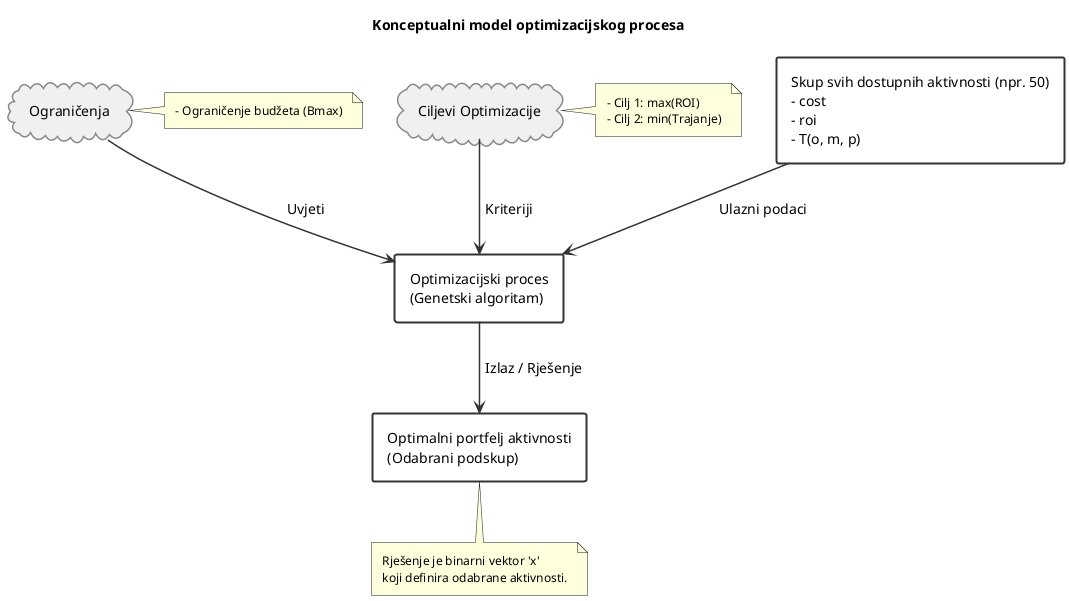
\includegraphics[width=0.8\textwidth]{slike/model_problema.png}
    \caption{Konceptualni model problema optimizacije portfelja projektnih aktivnosti.}
    \label{fig:konceptualni_model}
\end{figure}

Ovaj formalizirani model omogućuje jasnu matematičku i vizualnu reprezentaciju optimizacijskog zadatka. Precizna definicija ulaza, ograničenja i ciljeva ključna je za sustavnu primjenu optimizacijskih metoda poput genetskih algoritama \cite{Mitchell1998} u kombinaciji s Monte Carlo simulacijama \cite{Rubinstein2016}, kako bi se dobila rješenja visoke kvalitete koja su istovremeno i robusna na prisutne nesigurnosti.

\newpage

\section{Arhitektura sustava i implementacija}
\label{chap:implementacija}
Nakon definiranja teorijskih osnova i formalizacije problema, ovo poglavlje detaljno opisuje praktičnu realizaciju razvijenog optimizacijskog modela. Sustav je implementiran u programskom jeziku \textbf{Python (verzija 3.x)}, odabranom zbog čitljivosti, bogatog ekosustava biblioteka i široke primjene u znanstvenom računarstvu \cite{PythonSoftwareFoundation}. Python omogućuje brzu izradu prototipa, jednostavnu integraciju modula te učinkovitu obradu i vizualizaciju podataka.
\subsection{Korištene tehnologije i biblioteke}
Za izradu sustava korišten je niz standardnih biblioteka iz Python ekosustava za znanstveno računarstvo. Biblioteka \textbf{DEAP} \cite{DEAP2012} korištena je kao temeljni okvir za implementaciju genetskog algoritma. Za numeričke operacije i statističku obradu korišten je \textbf{NumPy} \cite{Harris2020}, dok je za manipulaciju i spremanje tabličnih podataka korišten \textbf{Pandas} \cite{PandasDevelopmentTeam2020}. Vizualizacija rezultata provedena je pomoću biblioteka \textbf{Seaborn} \cite{Waskom2021} i \textbf{Matplotlib} \cite{Hunter2007}. Modeliranje nesigurnosti pomoću Trokutaste distribucije implementirano je korištenjem standardne Python biblioteke Random. Detaljan pregled dan je u Tablici \ref{tab:biblioteke}.

\begin{table}[H]
\centering
\caption{Korištene biblioteke u implementaciji}
\label{tab:biblioteke}
\begin{tabular}{|l|p{10cm}|}
\hline
\textbf{Biblioteka} & \textbf{Namjena i citat} \\ \hline
Python & Osnovni programski jezik za cjelokupnu implementaciju. \cite{PythonSoftwareFoundation} \\ \hline
DEAP & Okvir za razvoj i provedbu evolucijskih algoritama. \cite{DEAP2012} \\ \hline
NumPy & Numeričke operacije i statistička obrada nizova podataka. \cite{Harris2020} \\ \hline
Pandas & Učitavanje, obrada i spremanje tabličnih podataka s rezultatima. \cite{PandasDevelopmentTeam2020} \\ \hline
Seaborn & Kreiranje naprednih statističkih vizualizacija (stupčasti, linijski i raspršeni grafikoni). \cite{Waskom2021} \\ \hline
Matplotlib & Osnovna biblioteka za crtanje na koju se oslanja Seaborn. \cite{Hunter2007} \\ \hline
Random & Standardna Python biblioteka korištena za generiranje slučajnih brojeva i uzorkovanje iz Trokutaste distribucije. \\ \hline
\end{tabular}
\end{table}

\subsection{Arhitektura eksperimentalnog okvira}

Sustav razvijen za potrebe ovog rada nije zamišljen kao monolitna skripta, već kao cjeloviti i modularni eksperimentalni okvir. Takva arhitektura, prikazana na Slici \ref{fig:tok_istrazivanja}, omogućuje sustavnu analizu, kalibraciju i usporedbu optimizacijskih metodologija. Okvir se sastoji od dva glavna analitička modula koji slijede dvo-fazni pristup istraživanju, te jednog pomoćnog modula za obradu i prikaz rezultata.

Prvi modul, \textbf{Modul za analizu i kalibraciju genetskog algoritma}, predstavlja temelj istraživanja i odgovara na pitanje: \emph{``Kako optimalno konfigurirati genetski algoritam za rješavanje zadanog problema?''}. Njegova primarna svrha je provođenje detaljne ablacijske studije kojom se ispituje utjecaj svakog ključnog parametra na performanse. Kroz višestruka pokretanja različitih konfiguracija (standardni GA, bez križanja, bez mutacije, s povećanim brojem generacija, s većom populacijom), izračunavanjem metrika performansi, uključujući prosječnu vrijednost (mean) i standardnu devijaciju (std) za ROI i procijenjeno trajanje, ovaj modul kao izlaz generira "šampionsku" konfiguraciju – skup optimalnih parametara koji osiguravaju najbolje performanse i koji se koriste u daljnjoj analizi.

    Drugi, ključni modul je \textbf{Modul za usporednu analizu optimizacijskih scenarija}. On čini srž diplomskog rada i koristi "šampionsku" konfiguraciju za provođenje konačne, statistički robusne usporedbe triju različitih pristupa rješavanju problema: osnovnog modela nasumične pretrage, klasičnog genetskog algoritma usmjerenog isključivo na ROI, te hibridnog GA+MC modela (NSGA-II) koji provodi više-kriterijsku optimizaciju koja istovremeno maksimizira ROI i minimizira rizik trajanja procijenjen Monte Carlo simulacijom.  Izlaz ovog modula je konačna tablica s usporednim rezultatima performansii(ROI, trajanje) i stabilnosti(standardna devijacija) za svaki od triju scenarija.

    Treći, \textbf{Modul za obradu i vizualizaciju rezultata}, služi kao pomoćni alat za interpretaciju podataka dobivenih iz prva dva modula, generirajući pregledne tablice i grafičke prikaze kao što su stupčasti dijagrami za usporedbu prosječnih vrijednosti ili 2D raspršeni dijagrami (scatter plots) za prikaz Paretovog fronta dobivenog iz NSGA-II algoritma generirane iz rezultata spremnjenih u CSV formatu.

\begin{figure}[H]
    \centering
    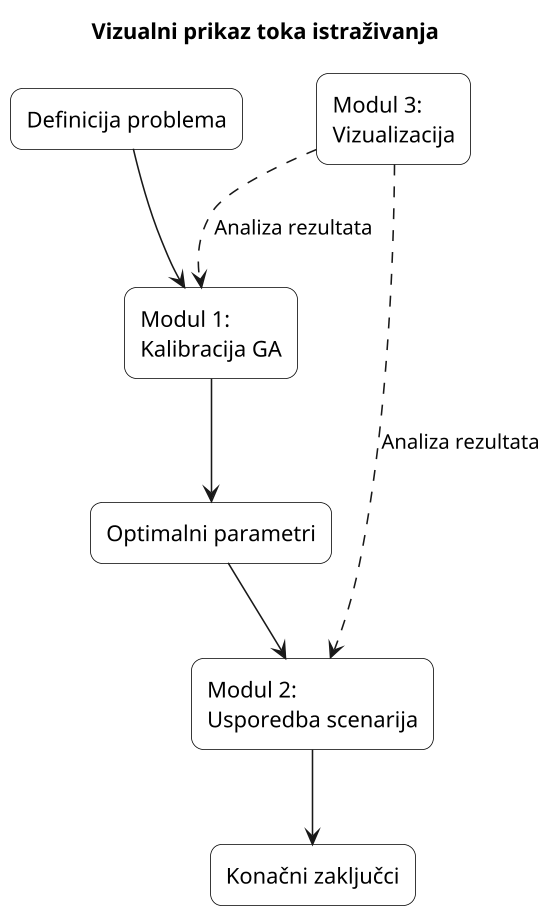
\includegraphics[width=0.9\textwidth]{slike/tijek_istrazivanja.png}
    \caption{Vizualni prikaz toka istraživanja}
    \label{tok istraživanja}
\end{figure}

\subsection{Modeliranje nesigurnosti: Monte Carlo simulacija}

Za svaku projektnu aktivnost definirane su tri točke procjene trajanja:
\[
a \ (\text{optimistična}), \quad
m \ (\text{najvjerojatnija}), \quad
b \ (\text{pesimistična})
\]
Iako u teoriji postoje kompleksnije distribucije poput \textit{Beta-PERT} distribucije, 
za potrebe ovog rada odabrana je \textbf{Trokutasta distribucija (Triangular distribution)} 
zbog svoje praktičnosti, računalne efikasnosti i intuitivnog temelja na tri poznate procjene.

\paragraph{Generiranje trajanja aktivnosti.}
U svakoj iteraciji Monte Carlo simulacije, trajanje svake aktivnosti generira se slučajnom vrijednošću 
unutar raspona $[a, b]$ s najvećom vjerojatnošću u točki $m$.  
Trokutasta distribucija definirana je funkcijom gustoće vjerojatnosti:
\[
f(x) =
\begin{cases}
\frac{2(x-a)}{(b-a)(m-a)}, & a \leq x < m, \\
\frac{2(b-x)}{(b-a)(b-m)}, & m \leq x \leq b, \\
0, & \text{inače}.
\end{cases}
\]

\paragraph{Procjena trajanja portfelja.}
Ukupno trajanje projektnog portfelja u jednoj simulaciji dobiva se zbrojem trajanja svih aktivnosti odabranih u tom portfelju:
\[
T_{\text{portfolio}} = \sum_{i \in S} t_i
\]
gdje je $S$ skup odabranih aktivnosti, a $t_i$ generirano trajanje aktivnosti $i$.

Implementacija se temelji na \texttt{monte\_carlo\_eval\_duration} funkciji.
\begin{lstlisting}[language=Python, caption={Funkcija za Monte Carlo procjenu trajanja}, label={lst:monte_carlo}, captionpos=b]
def monte_carlo_eval_duration(individual, activities, config):
    selected = [act for i, act in enumerate(activities) if individual[i] == 1]
    if not selected:
        return 0.0
    durations = [
        sum(
            random.triangular(act["optimistic"], act["realistic"], act["pessimistic"])
            for act in selected
        )
        for _ in range(config["NUM_SIMULATIONS"])
    ]
    return np.mean(durations)
\end{lstlisting}


\paragraph{Agregiranje rezultata.}
Monte Carlo simulacija ponavlja se velik broj puta $(\text{NUM\_SIMULATIONS})$, a konačna procjena trajanja portfelja 
dobiva se kao prosječna vrijednost svih simuliranih trajanja:
\[
\overline{T}(S) = \frac{1}{\text{NUM\_SIMULATIONS}} \sum_{k=1}^{\text{NUM\_SIMULATIONS}} T_{\text{portfolio}}^{(k)}
\]
gdje $T_{\text{portfolio}}^{(k)}$ označava ukupno trajanje portfelja u $k$-toj simulaciji.


\subsection{Optimizacijski pristup: Genetski algoritam}

Implementacija genetskog algoritma provedena je pomoću programske biblioteke \texttt{DEAP} (Distributed Evolutionary Algorithms in Python) \cite{DEAP2012}. 
S obzirom na prirodu problema odabira podskupa aktivnosti, korištena je \textbf{binarna reprezentacija}, gdje svaka jedinka (kromosom) predstavlja jedan portfelj projekata u obliku binarnog niza. Vrijednost '1' na poziciji i označava da je $i$-ta aktivnost odabrana, dok '0' označava da nije.
\paragraph{Reprezentacija jedinke.}
Svaka jedinka (kromosom) u populaciji predstavlja jedno potencijalno rješenje – jedan portfelj projekata. 
Predstavljena je kao binarni niz duljine jednake ukupnom broju aktivnosti $(\text{NUM\_ACTIVITIES})$, gdje gen na poziciji $i$ ima vrijednost:
\[
g_i =
\begin{cases}
1, & \text{ako je $i$-ta aktivnost odabrana}, \\
0, & \text{ako nije odabrana}.
\end{cases}
\]

\paragraph{Funkcija pogodnosti (Fitness Function).}
Ključni dio implementacije su funkcije pogodnosti. Ovisno o scenariju, korištene su dvije različite funkcije. Za jedno-kriterijsku optimizaciju (GA samo ROI), implementirana je funkcija koja maksimizira ROI i primjenjuje strogu kaznenu metodu za rješenja koja prekoračuju budžet, osiguravajući da su sva nevaljana rješenja lošija od bilo kojeg valjanog.
Za hibridni scenarij (GA+MC), implementirana je više-kriterijska funkcija pogodnosti koja predstavlja srž ovog rada. Kao što je prikazano u Isječku koda \ref{lst:fitness_function}, ova funkcija unutar jedne evaluacije objedinjuje deterministički izračun (ukupni trošak i ROI) i poziv stohastičke Monte Carlo simulacije za procjenu rizika (očekivano trajanje). Vraća tuple s dvije vrijednosti, omogućujući NSGA-II algoritmu da istovremeno optimizira oba cilja.
\begin{figure}
    \centering
\begin{lstlisting}[language=Python, caption={Više-kriterijska funkcija pogodnosti}, label={lst:fitness_function}, captionpos=b ]
def multi_objective_fitness(individual, activities, config):
    total_cost, total_roi = calculate_metrics(individual, activities)
    if total_cost > config["BUDGET"]:
        return 0, 99999
    avg_duration = monte_carlo_eval_duration(individual, activities, config)
    return total_roi, avg_duration
\end{lstlisting}
\end{figure}
Ovisno o eksperimentalnom scenariju, korištene su dvije vrste funkcije pogodnosti:
\begin{enumerate}
    \item \textbf{Jedno-kriterijska optimizacija.}  
Za scenarij GA (samo ROI), cilj je bio isključivo maksimizacija ukupnog povrata na investiciju (ROI). Za rukovanje ograničenjem budžeta primijenjena je stroga kaznena metoda. Ako ukupni trošak odabranog portfelja $S$ ne prelazi budžet, njegova pogodnost je jednaka ukupnom ROI-u. U suprotnom, pogodnost postaje negativna vrijednost proporcionalna iznosu prekoračenja:
$$
\text{Fitness}(S) = 
\begin{cases}
    \sum_{i \in S} \text{ROI}_i, & \text{ako } \sum_{i \in S} \text{Trošak}_i \leq \text{Budžet} \\
    -\left(\sum_{i \in S} \text{Trošak}_i - \text{Budžet}\right), & \text{ako } \sum_{i \in S} \text{Trošak}_i > \text{Budžet}
\end{cases}
$$
Ovakav pristup osigurava da svako valjano rješenje (koje ima pozitivan fitness) uvijek bude ocijenjeno kao bolje od bilo kojeg nevaljanog rješenja (koje ima negativan fitness).    \item \textbf{Više-kriterijska optimizacija.}  
    Za hibridni scenarij \texttt{GA+MC} korišten je napredni algoritam NSGA-II, s ciljem istovremene optimizacije dva suprotstavljena kriterija:
    \begin{enumerate}
        \item maksimizirati ROI,
        \item minimizirati prosječno trajanje projekta, procijenjeno Monte Carlo simulacijom.
    \end{enumerate}
    Formalno:
    \[
    \begin{cases}
    \max f_1(S) = ROI(S) \\
    \min f_2(S) = \overline{T}(S)
    \end{cases}
    \]
    gdje $\overline{T}(S)$ označava prosječno trajanje portfelja $S$.
\end{enumerate}

\paragraph{Genetski operatori.}
Za evoluciju populacije korišteni su sljedeći standardni genetski operatori za binarnu reprezentaciju koje pruža DEAP. Za \textbf{Selekciju} su primijenjeni Turnirska selekcija (\texttt{tools.selTournament}) za jedno-kriterijsku optimizaciju, te \texttt{tools.selNSGA2} za više-kriterijsku optimizaciju. Kao operator \textbf{križanja} korišteno je križanje u dvije točke (\texttt{tools.cxTwoPoint}), koje razmjenjuje segmente između dva roditeljska kromosoma, dok je za \textbf{mutaciju} korištena slučajna promjena bita (\texttt{tools.mutFlipBit}), koja s malom vjerojatnošću mijenja vrijednost pojedinog gena (iz $0$ u $1$ ili obrnuto), osiguravajući genetsku raznolikost i sprječavajući preranu konvergenciju.

\subsection{Vizualizacija i obrada rezultata}

Za analizu i prikaz rezultata dobivenih optimizacijom korištene su biblioteke \texttt{pandas} za tabličnu obradu podataka te \texttt{Seaborn} i \texttt{Matplotlib} \cite{Waskom2021, Hunter2007} za grafičku vizualizaciju.
Ovaj pristup omogućio je sustavnu prezentaciju statistički obrađenih podataka kroz detaljne tablice te vizualnu usporedbu modela pomoću stupčastih i raspršenih dijagrama. Posebno je značajan prikaz Paretovog fronta, koji jasno ilustrira kompromis (trade-off) između maksimizacije ROI-a i minimizacije trajanja, pružajući intuitivan uvid u kvalitetu rješenja dobivenih više-kriterijskom optimizacijom.

Kombinacija alata omogućila je jasnu i preglednu prezentaciju rezultata 
dobivenih iz eksperimentalnih scenarija.

Ključni vizualni elementi korišteni u ovom radu uključuju:

    \textbf{Tablične prikaze:} Detaljne tablice s konačnim, statistički obrađenim rezultatima 
    usporedbe različitih optimizacijskih scenarija, uključujući osnovne metrike 
    poput prosječnog ROI-a, prosječnog trajanja te raspona vrijednosti.

    \textbf{Stupčaste dijagrame:} Koristili su se za vizualnu usporedbu prosječnih vrijednosti 
    (\textit{ROI} i trajanje) između različitih metodologija optimizacije, omogućujući brzu identifikaciju 
    učinkovitijih pristupa.

    \textbf{Raspršene dijagrame (Scatter Plot):} Prikaz Paretovog fronta dobivenog NSGA-II algoritmom, 
    koji jasno ilustrira kompromis (\textit{trade-off}) između dvaju suprotstavljenih ciljeva:
    maksimizacije ROI-a i minimizacije trajanja. Time se omogućuje intuitivna procjena 
    učinkovitosti rješenja.

Vizualizacija rezultata odigrala je ključnu ulogu u interpretaciji dobivenih podataka, 
posebno u scenarijima s više ciljeva, gdje tablični prikazi sami po sebi nisu dovoljni 
za uočavanje odnosa i kompromisa među varijablama.


\newpage


\section{Eksperimentalna evaluacija i diskusija rezultata}
\label{chap:eksperimenti}

U ovom poglavlju detaljno se opisuje eksperimentalni postav, provedba eksperimenata te dubinska analiza i interpretacija dobivenih rezultata. Cilj je bio empirijski validirati predloženi hibridni model, kvantificirati njegove performanse i usporediti ga s drugim relevantnim pristupima kako bi se donijeli utemeljeni zaključci o njegovoj primjenjivosti.

\subsection{Postavke okruženja i testni podaci}
Svi eksperimenti provedeni su u programskom okruženju \textbf{Python (verzija 3.x)} na standardnom osobnom računalu. Kako bi se osigurala ponovljivost i kontrolirani uvjeti, za potrebe istraživanja generiran je sintetički skup podataka koji oponaša realističan projektni portfelj. U ovisnosti o eksperimentalnoj seriji, broj jedinstvenih projektnih aktivnosti varirao je od 10 do 100. Svaka aktivnost je parametrizirana slučajnim vrijednostima unutar zadanih raspona, uključujući \textbf{Trošak (\texttt{cost}):} slučajna cjelobrojna vrijednost između 50 i 200, \textbf{ROI (\texttt{roi}):} slučajna decimalna vrijednost između 1.0 i 3.0, i \textbf{Procjene trajanja:} optimistično (između 5 i 10 dana), najvjerojatnije (između 10 i 20 dana) i pesimistično (između 20 i 40 dana).
Ukupni raspoloživi budžet za portfelj (\texttt{BUDGET}) bio je skaliran u skladu sa složenošću problema.

\subsection{Eksperimentalni dizajn}
Kako bi se osigurala metodološka ispravnost i izbjegli proizvoljni zaključci, istraživanje je provedeno kroz dvo-fazni eksperimentalni proces:
\begin{itemize}
    \item \textbf{Faza 1: Analiza i kalibracija genetskog algoritma.} U prvoj fazi provedena je detaljna ablacijska studija kako bi se utvrdilo koji parametri genetskog algoritma daju najkvalitetnija i najstabilnija rješenja za reprezentativni tip problema (50 aktivnosti). Cilj je bio pronaći ``šampionsku'' konfiguraciju GA.
    \item \textbf{Faza 2: Usporedna analiza optimizacijskih modela.} U drugoj fazi, ``šampionska'' konfiguracija GA, dobivena u prvoj fazi, korištena je kao osnova za provođenje konačne usporedbe triju različitih optimizacijskih scenarija i evaluaciju glavnih hipoteza rada na problemima različite skale i restriktivnosti.
\end{itemize}

\subsubsection{Istraživačke hipoteze}
Na temelju teorijske podloge i postavljenih istraživačkih pitanja iz Uvoda, definirane su sljedeće tri glavne hipoteze koje se provjeravaju kroz eksperimente:

\begin{description}
    \item[H1 (Hipoteza o Skalabilnosti):] Povećanjem složenosti problema (broja aktivnosti), performanse modela temeljenog na nasumičnoj pretrazi (Random Search) će se značajno smanjiti u usporedbi s modelima temeljenim na genetskim algoritmima.
    \item[H2 (Hipoteza o Kompromisu):] Hibridni `GA+MC` model će, za razliku od klasičnog `GA (samo ROI)` modela, uspješno identificirati rješenja koja predstavljaju superioran kompromis između profitabilnosti (ROI) i rizika (trajanje projekta), posebno na problemima veće složenosti.
    \item[H3 (Hipoteza o Utjecaju Ograničenja):] Restriktivnost problema, specifično kroz promjenu raspoloživog budžeta, značajno utječe na performanse i stabilnost optimizacijskih modela, pri čemu se očekuje da će ekstremna ograničenja predstavljati najveći izazov za najsloženije modele.
\end{description}

\subsection{Eksperiment 1: Analiza parametara i kalibracija genetskog algoritma}

Prvi eksperiment imao je za cilj empirijski provjeriti utjecaj osnovnih genetskih operatora i parametara na performanse algoritma te odabrati optimalnu konfiguraciju za daljnje testiranje. U tu svrhu provedena je ablacijska studija s pet različitih konfiguracija, gdje je svaka pokrenuta 10 puta (\texttt{RUNS = 10}) radi statističke pouzdanosti. Testirane konfiguracije su bile: \emph{Standardni GA}, \emph{Bez mutacije}, \emph{Bez križanja}, \emph{Više generacija} i \emph{Veća populacija}.

\subsubsection{Rezultati i diskusija} Rezultati ablacijske studije prikazani su u Tablici~\ref{tab:ga_ablation} te grafički na Slici~\ref{fig:ga_ablation}.

\begin{table}[H]
    \centering
    \caption{Rezultati ablacijske studije za parametre GA.}
    \label{tab:ga_ablation}
    \begin{tabular}{|l|c|c|c|c|}
        \hline
        \textbf{Postavka} & \textbf{ROI\_mean} & \textbf{ROI\_std} & \textbf{Trajanje\_mean} & \textbf{Trajanje\_std} \\
        \hline
        Standardni GA & 28.985 & 1.543 & 199.216 & 10.691 \\
        Bez mutacije & 27.627 & 1.581 & 193.497 & 11.364 \\
        Bez križanja & 25.884 & 1.865 & 191.514 & 9.174 \\
        Više generacija & 31.183 & 0.928 & 205.026 & 13.649 \\
        \textbf{Veća populacija} & \textbf{31.683} & \textbf{0.720} & \textbf{213.694} & \textbf{5.574} \\
        \hline
    \end{tabular}
\end{table}

Analiza rezultata potvrđuje obje početne hipoteze i ključnu ulogu genetskih operatora. Uklanjanje križanja drastično smanjuje performanse, potvrđujući da je rekombinacija dobrih rješenja ključan mehanizam pretrage. S druge strane, povećanje računalnih resursa, bilo kroz više generacija (dubina pretrage) ili veću populaciju (širina pretrage), dovodi do superiornih i statistički stabilnijih rješenja. Konfiguracija \emph{Veća populacija} pokazala se najboljom, ostvarivši najviši prosječni ROI uz najnižu standardnu devijaciju. Zanimljivo je primijetiti da konfiguracije s najvišim ROI-em rezultiraju i najdužim prosječnim trajanjem, što stvara prirodni kompromis (\emph{trade-off}) između profita i rizika, koji će biti predmet analize u sljedećem eksperimentu.

\begin{figure}[H]
    \centering
    \begin{subfigure}[b]{0.48\textwidth}
        \centering
        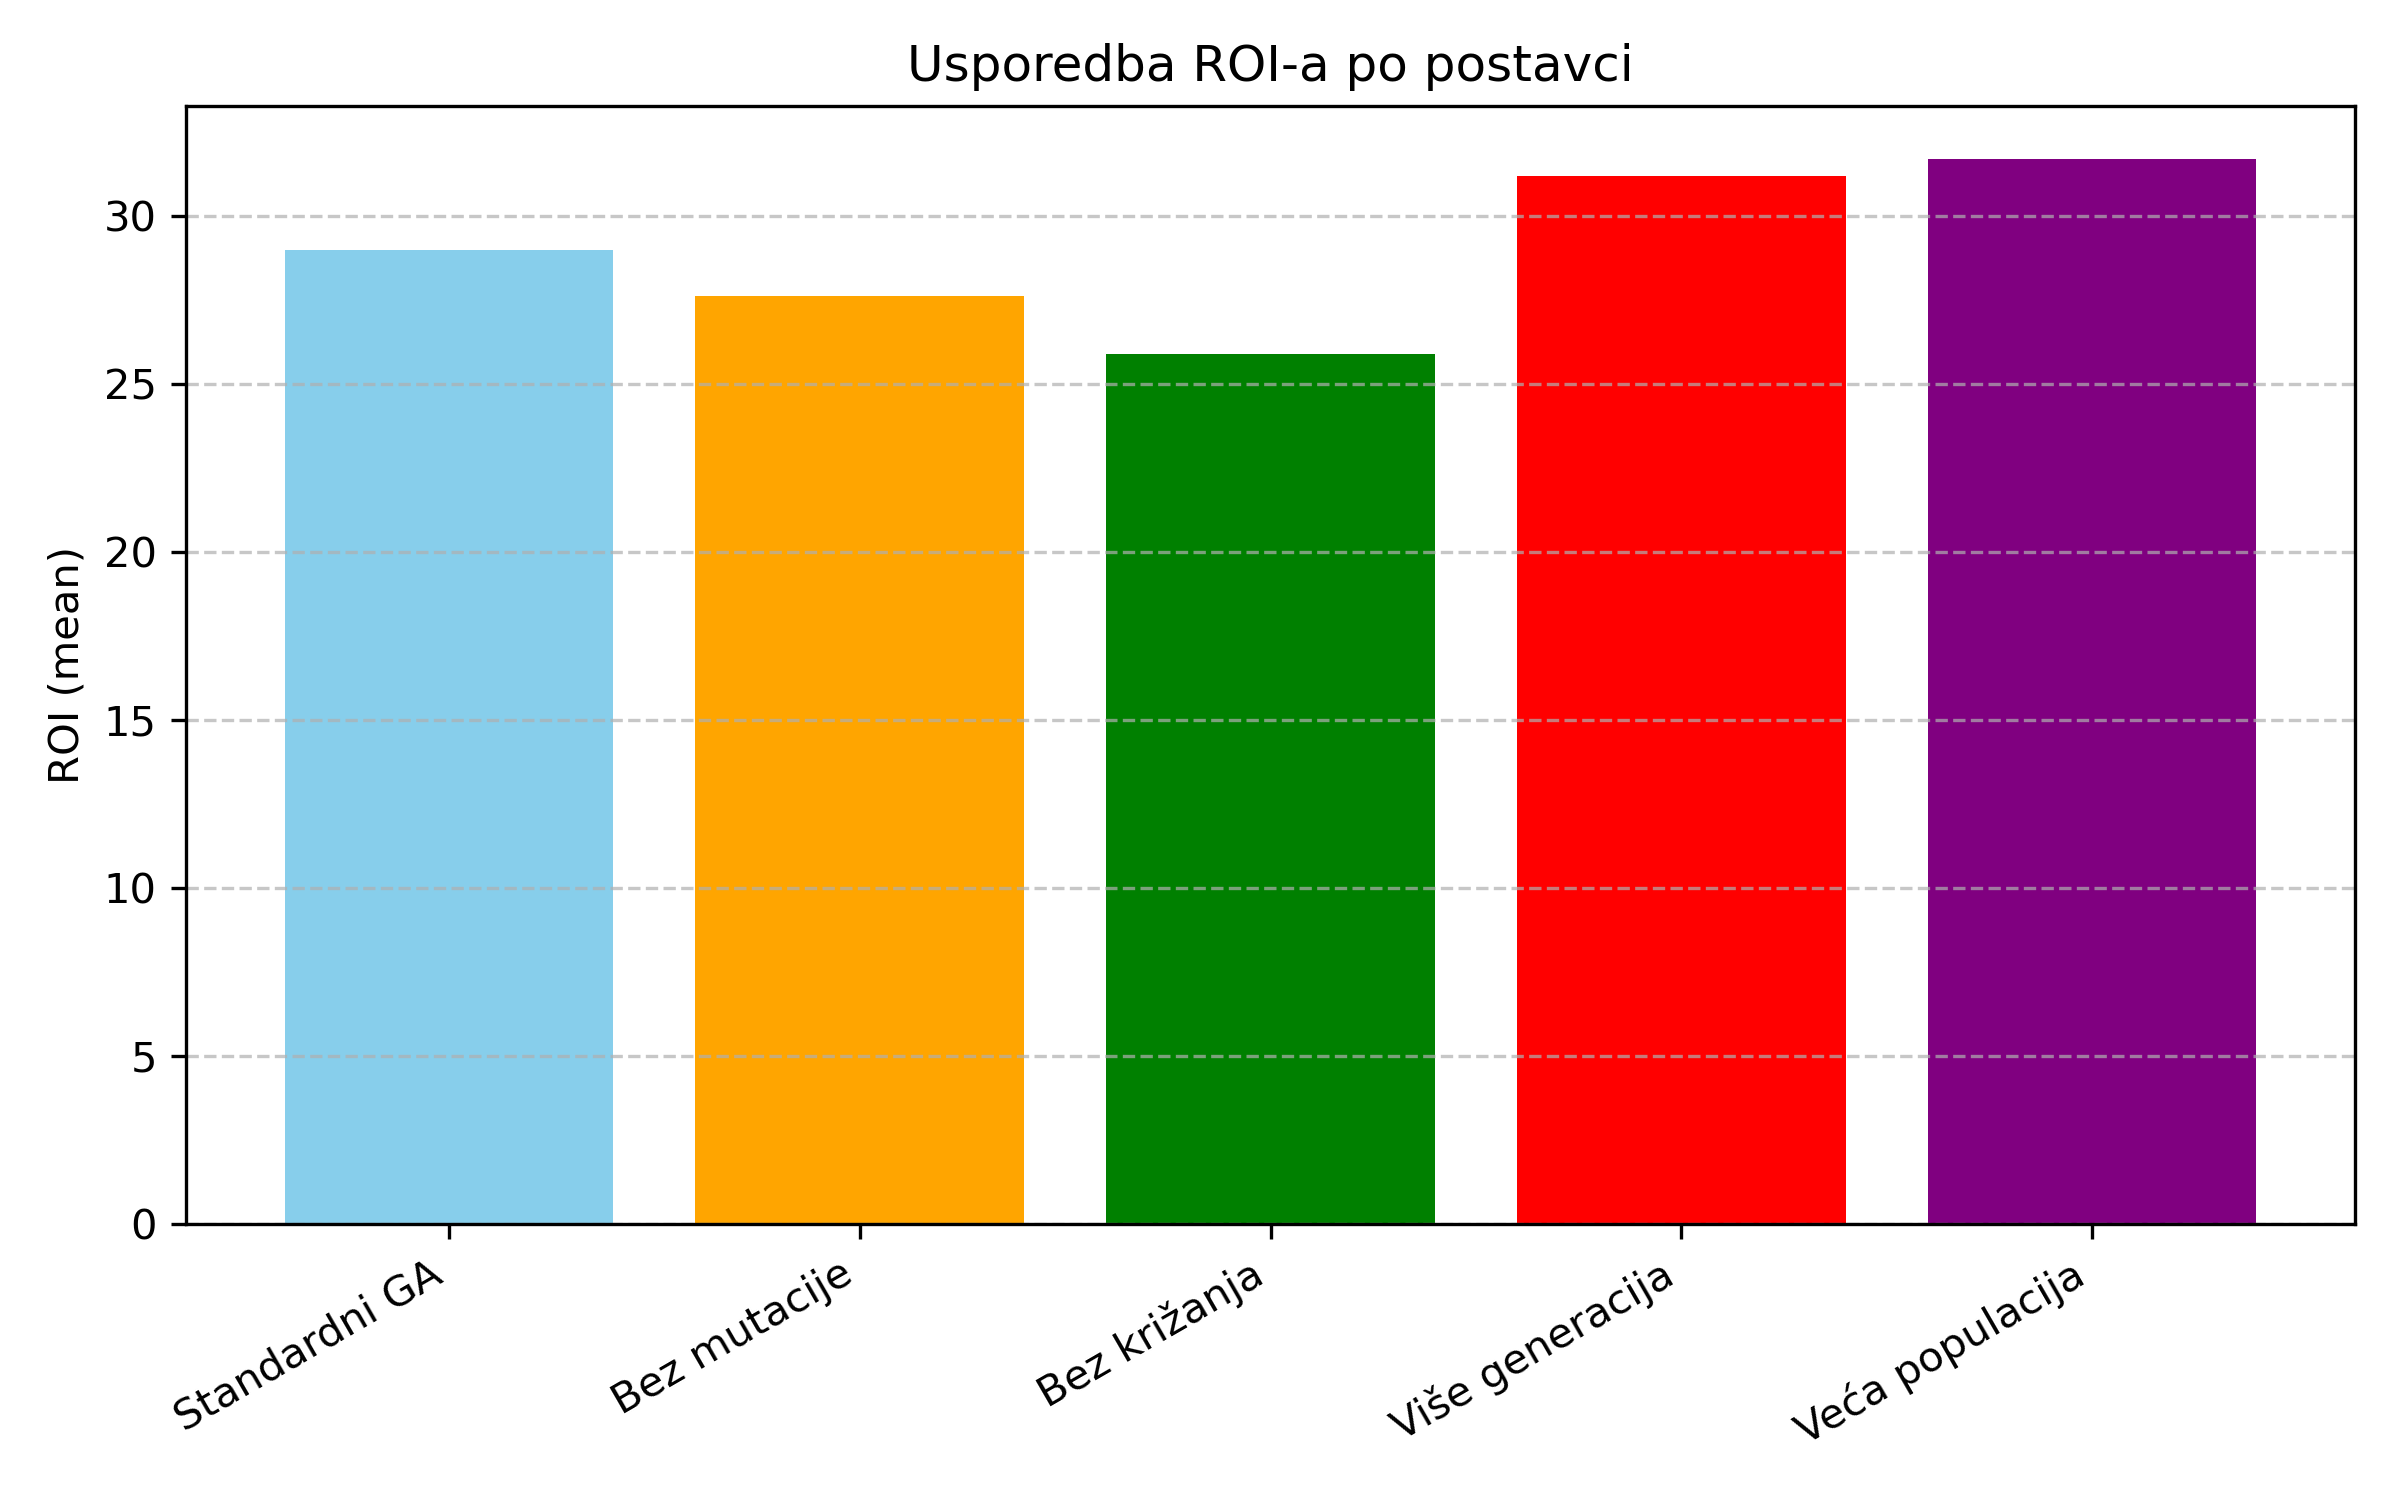
\includegraphics[width=\textwidth]{slike/ga_usporedba_roi.png}
        \caption{Usporedba prosječnog ROI-a.}
        \label{fig:ga_roi}
    \end{subfigure}
    \hfill
    \begin{subfigure}[b]{0.48\textwidth}
        \centering
        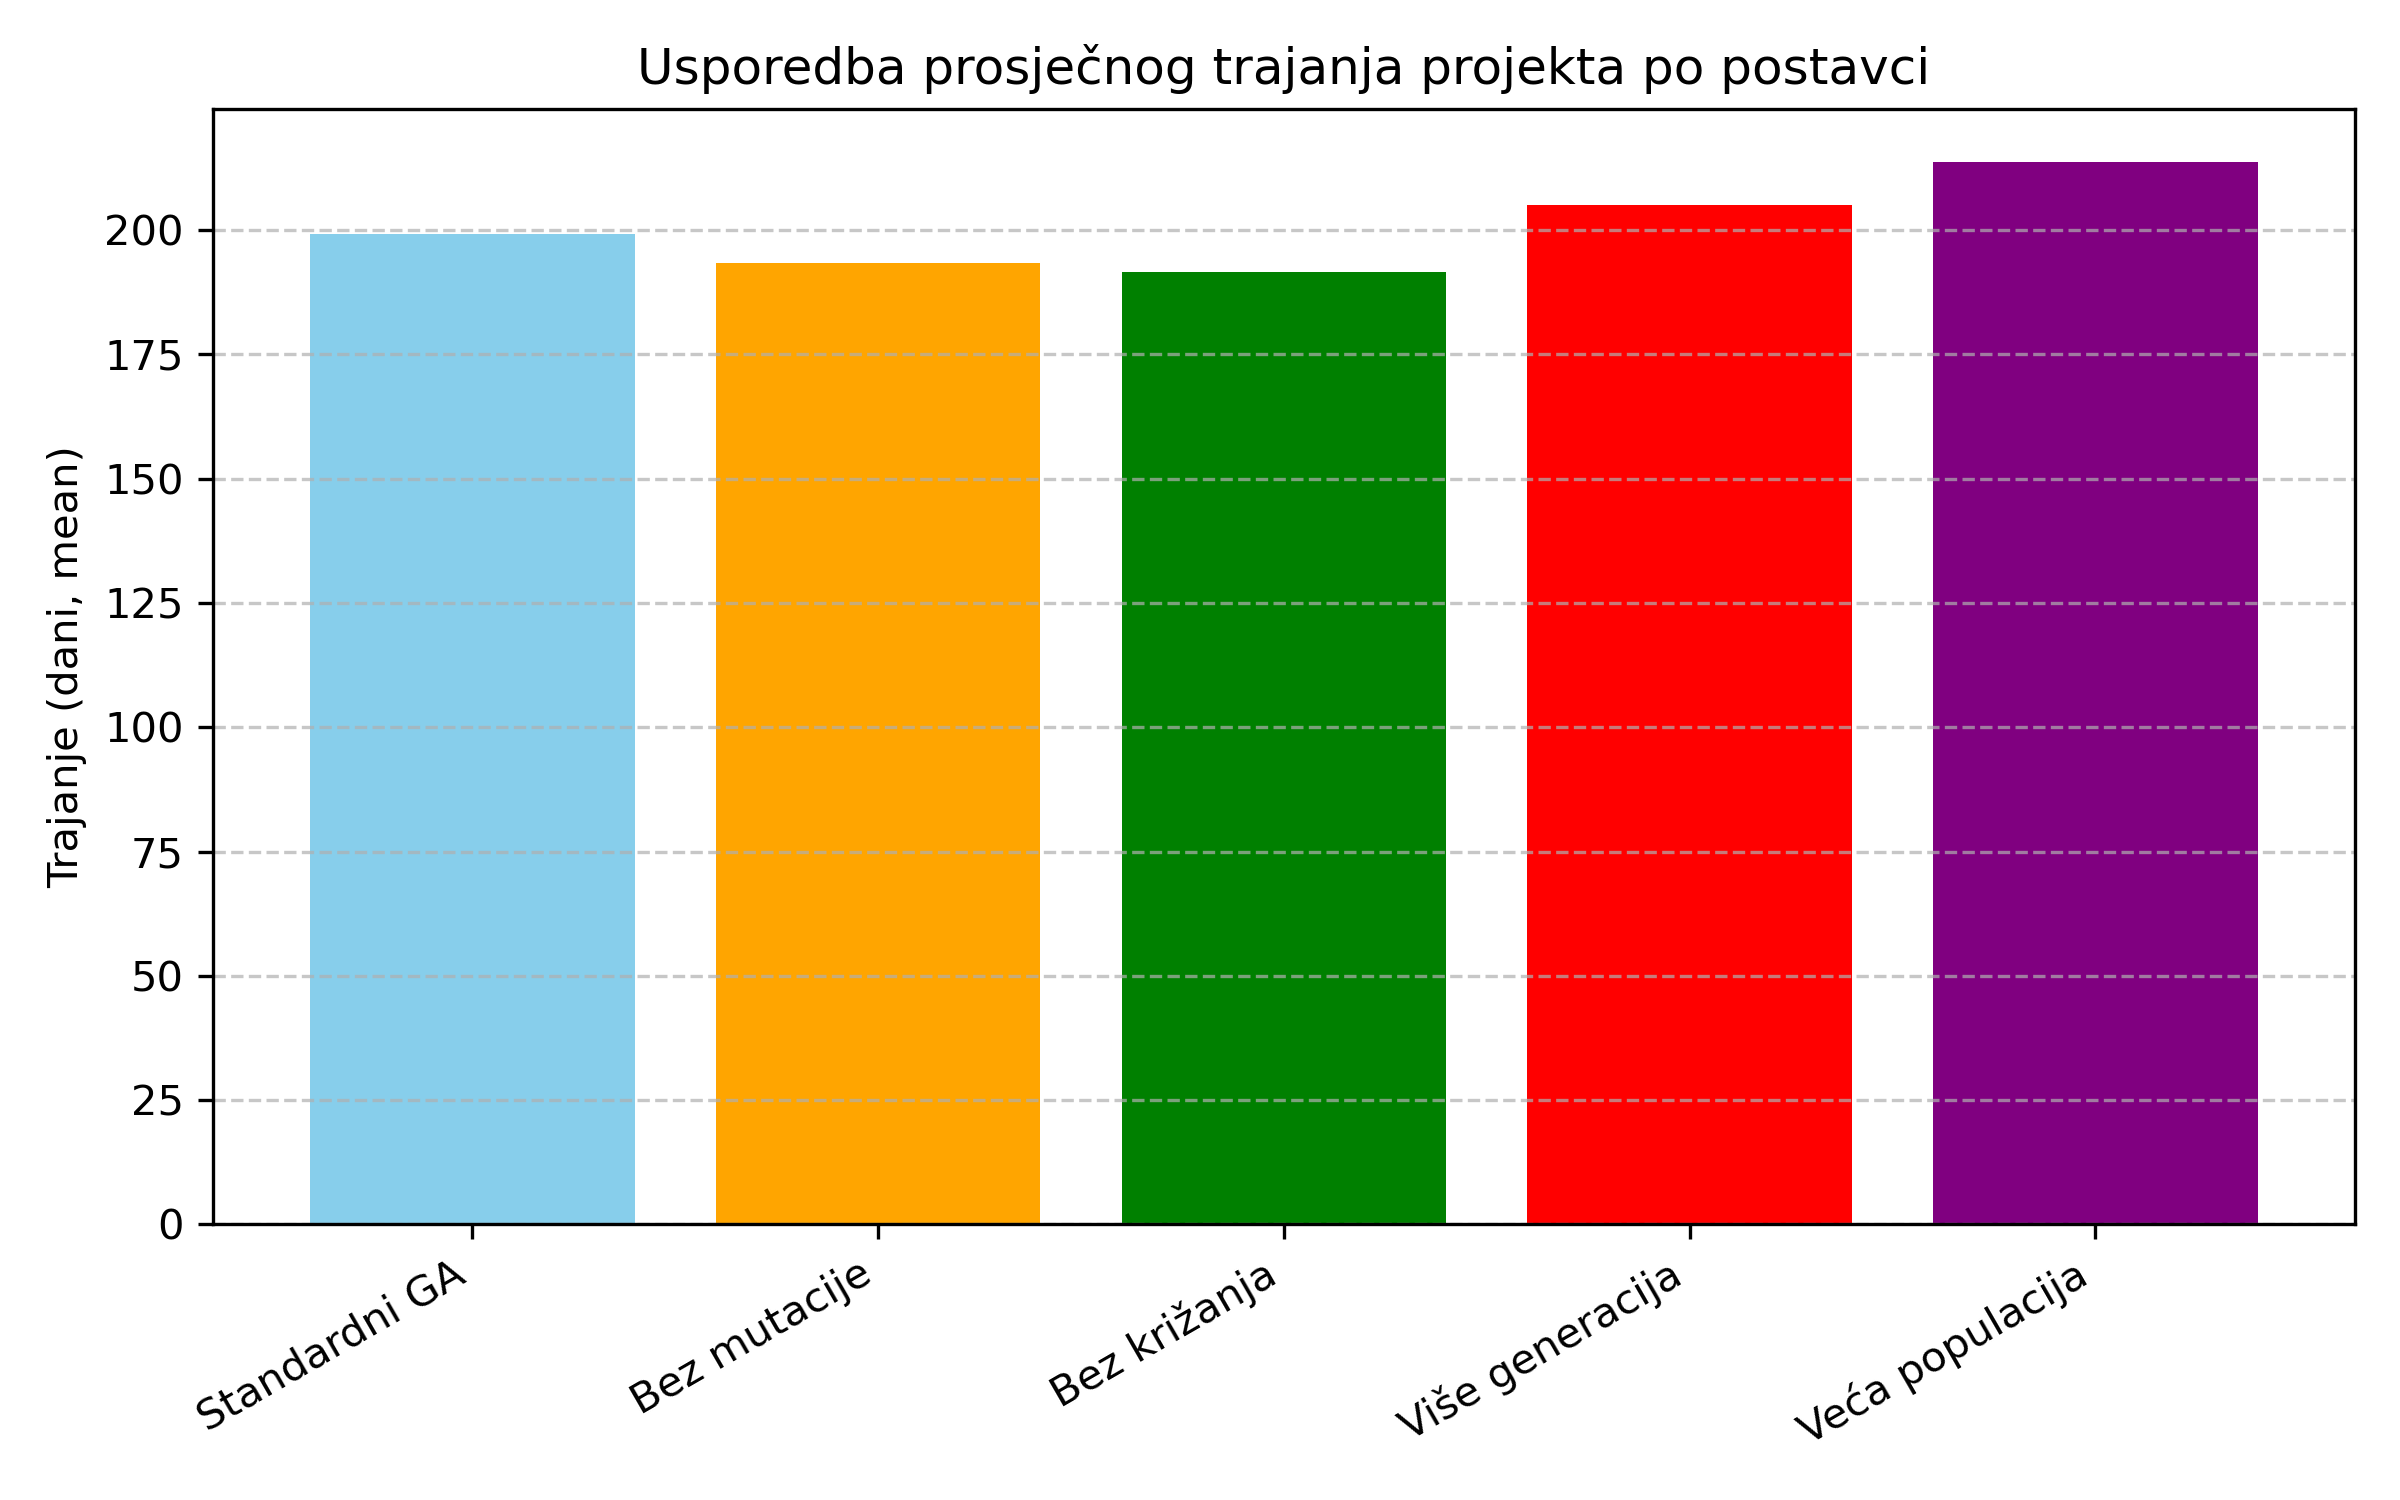
\includegraphics[width=\textwidth]{slike/ga_usporedba_trajanje.png}
        \caption{Usporedba prosječnog trajanja.}
        \label{fig:ga_trajanje}
    \end{subfigure}
    \caption{Grafički prikaz rezultata ablacijske studije za genetski algoritam.}
    \label{fig:ga_ablation}
\end{figure}

Na temelju empirijskih rezultata, konfiguracija \emph{Veća populacija} odabrana je kao ``šampionska''. Njezini parametri (\texttt{POP\_SIZE = 200}, \texttt{NGEN = 40}, itd.) poslužili su kao osnova za definiranje parametara u drugoj fazi istraživanja, uz nužne prilagodbe resursa s obzirom na složenost problema.

\subsection{Eksperiment 2: Usporedna analiza optimizacijskih modela}
Druga faza istraživanja čini ključnu eksperimentalnu provjeru glavne hipoteze rada. Koristeći kalibrirane parametre iz Eksperimenta 1, provedena je sustavna usporedba triju razvijenih modela. Cilj drugog eksperimenta je empirijski provjeriti postavljene istraživačke hipoteze (h1, h2, h3) kroz sustavnu usporedbu performansi, robusnosti i stabilnosti triju razvijenih modela: nasumične pretrage, jedno-kriterijskog GA i više-kriterijskog hibridnog GA+MC modela. usporedba je provedena na problemima različite skale i restriktivnosti prema planu definiranom u tablici~\ref{tab:plan_eksperimenata}. svaki od pet jedinstvenih eksperimentalnih scenarija pokrenut je 10 puta (\texttt{RUNS = 10}) radi osiguravanja statističke pouzdanosti. modeli koji koriste genetski algoritam (`GA (samo ROI)` i `GA+MC (NSGA-II)`) temeljili su se na ``šampionskoj'' konfiguraciji utvrđenoj u eksperimentu 1, uz skaliranje parametra `NGEN` sukladno složenosti problema.

\begin{table}[H]
    \centering
    \caption{Plan naprednih eksperimenata.}
    \label{tab:plan_eksperimenata}
    \resizebox{\textwidth}{!}{
    \begin{tabular}{|l|l|l|l|l|}
        \hline
        \textbf{Eksperiment} & \textbf{NUM\_ACTIVITIES} & \textbf{BUDGET} & \textbf{Pripada seriji} & \textbf{Napomena} \\
        \hline
        A1 & 10 & 1000 & A & Osnovna složenost \\
        \hline
        A2 / B2 & 50 & 2500 & A, B & Centralni / Referentni eksperiment \\
        \hline
        A3 & 100 & 5000 & A & Visoka složenost \\
        \hline
        B1 & 50 & 1500 & B & Restriktivan budžet \\
        \hline
        B3 & 50 & 4000 & B & Labav budžet \\
        \hline
    \end{tabular}
    }
\end{table}

\subsubsection{Rezultati i diskusija}
Svi rezultati dobiveni provođenjem Eksperimenta 2 sažeti su u Tablici~\ref{tab:rezultati}. U nastavku slijedi detaljna diskusija ovih rezultata, organizirana po tematskim cjelinama koje odgovaraju postavljenim hipotezama. Ova tablica predstavlja temelj za daljnju diskusiju.

\begin{table}[H]
    \centering
    \caption{Konačni rezultati usporedne analize optimizacijskih modela.}
    \label{tab:rezultati}
    \resizebox{\textwidth}{!}{
    \begin{tabular}{|l|l|c|c|c|c|}
        \hline
        \textbf{Eksperiment} & \textbf{Scenarij} & \textbf{ROI\_mean} & \textbf{ROI\_std} & \textbf{Trajanje\_mean} & \textbf{Trajanje\_std} \\
        \hline
        A1\_Osnovni & Random Search (MC) & 17.140 & 3.55e-15 & 144.151 & 0.911 \\
        A1\_Osnovni & GA (samo ROI) & 17.140 & 3.55e-15 & 143.103 & 1.239 \\
        A1\_Osnovni & GA+MC (NSGA-II) & 17.140 & 3.55e-15 & 142.003 & 0.372 \\
        \hline
        A2\_Srednji & Random Search (MC) & 40.108 & 0.703 & 341.024 & 9.405 \\
        A2\_Srednji & GA (samo ROI) & 46.125 & 0.412 & 363.632 & 7.843 \\
        A2\_Srednji & GA+MC (NSGA-II) & 44.099 & 0.980 & 319.210 & 13.171 \\
        \hline
        A3\_Slozeni & Random Search (MC) & 95.835 & 1.468 & 715.604 & 10.451 \\
        A3\_Slozeni & GA (samo ROI) & 114.224 & 0.891 & 792.300 & 11.933 \\
        A3\_Slozeni & GA+MC (NSGA-II) & 109.095 & 2.008 & 681.565 & 21.733 \\
        \hline
        B1\_Restriktivan & Random Search (MC) & 24.120 & 1.846 & 197.621 & 20.181 \\
        B1\_Restriktivan & GA (samo ROI) & 37.976 & 0.567 & 253.562 & 12.386 \\
        B1\_Restriktivan & GA+MC (NSGA-II) & 17.711 & 17.728 & 50104.382 & 49894.619 \\
        \hline
        B3\_Labav & Random Search (MC) & 71.379 & 1.114 & 536.901 & 16.247 \\
        B3\_Labav & GA (samo ROI) & 79.065 & 0.518 & 562.191 & 9.345 \\
        B3\_Labav & GA+MC (NSGA-II) & 76.949 & 0.487 & 526.612 & 10.602 \\
        \hline
    \end{tabular}
    }
\end{table}

Dobiveni rezultati analizirani su kroz tematske cjeline, s ciljem odgovaranja na postavljena istraživačka pitanja.

\textbf{Analiza Skalabilnosti (Serija A)}
Kao što je vidljivo na Slici~\ref{fig:a_skalabilnost}, porast složenosti problema drastično utječe na performanse modela. Jaz u \textbf{ROI\_mean} vrijednostima eksponencijalno raste u korist genetskih algoritama, potvrđujući hipotezu o nužnosti inteligentne pretrage (H1). Ovakav nalaz, gdje metaheuristički pristupi značajno nadmašuju nasumičnu pretragu na složenim problemima, u skladu je s rezultatima koje su dobili i drugi istraživači u srodnim domenama primjene \cite{Gandomi2013}. Istovremeno, analiza trajanja otkriva postojanje kompromisa: hibridni model GA+MC (NSGA-II) konzistentno identificira rješenja sa značajno nižim prosječnim trajanjem, potvrđujući hipotezu H2.

\begin{figure}[H]
    \centering
    \begin{subfigure}[b]{0.48\textwidth}
        \centering
        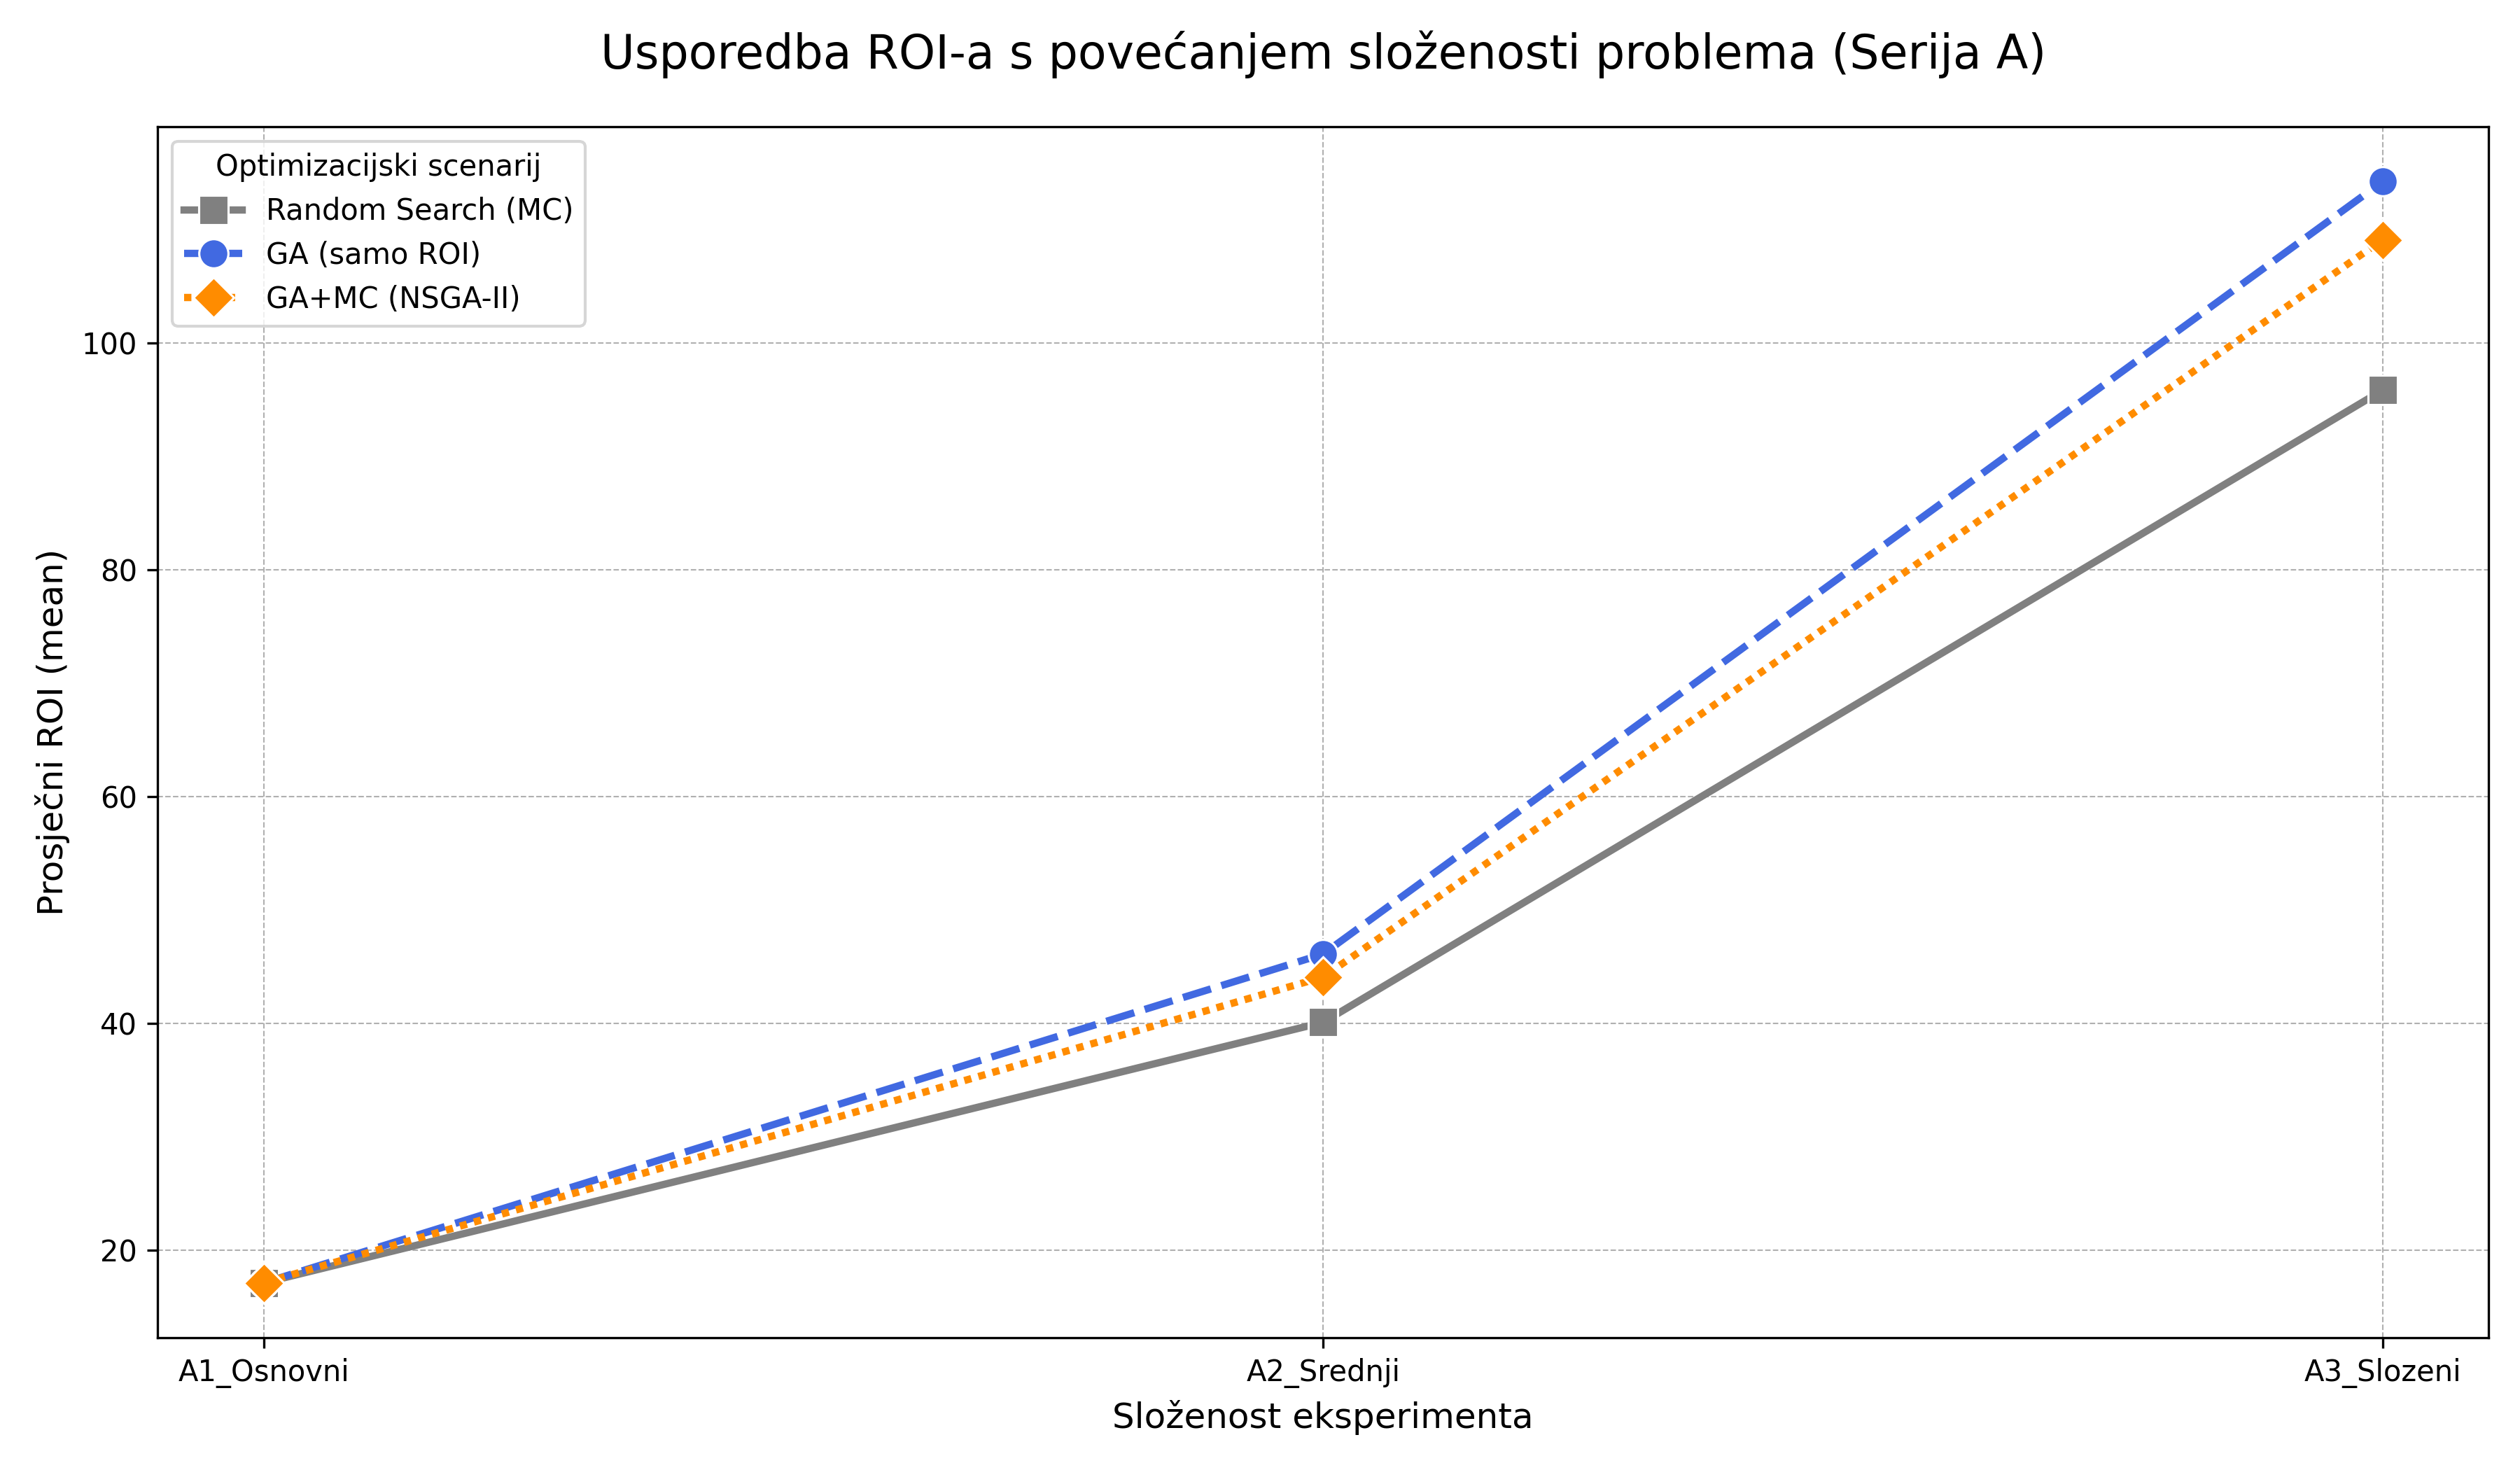
\includegraphics[width=\textwidth]{slike/grafikoni_final/A_skalabilnost_roi.png}
        \caption{Usporedba prosječnog ROI-a.}
    \end{subfigure}
    \hfill
    \begin{subfigure}[b]{0.48\textwidth}
        \centering
        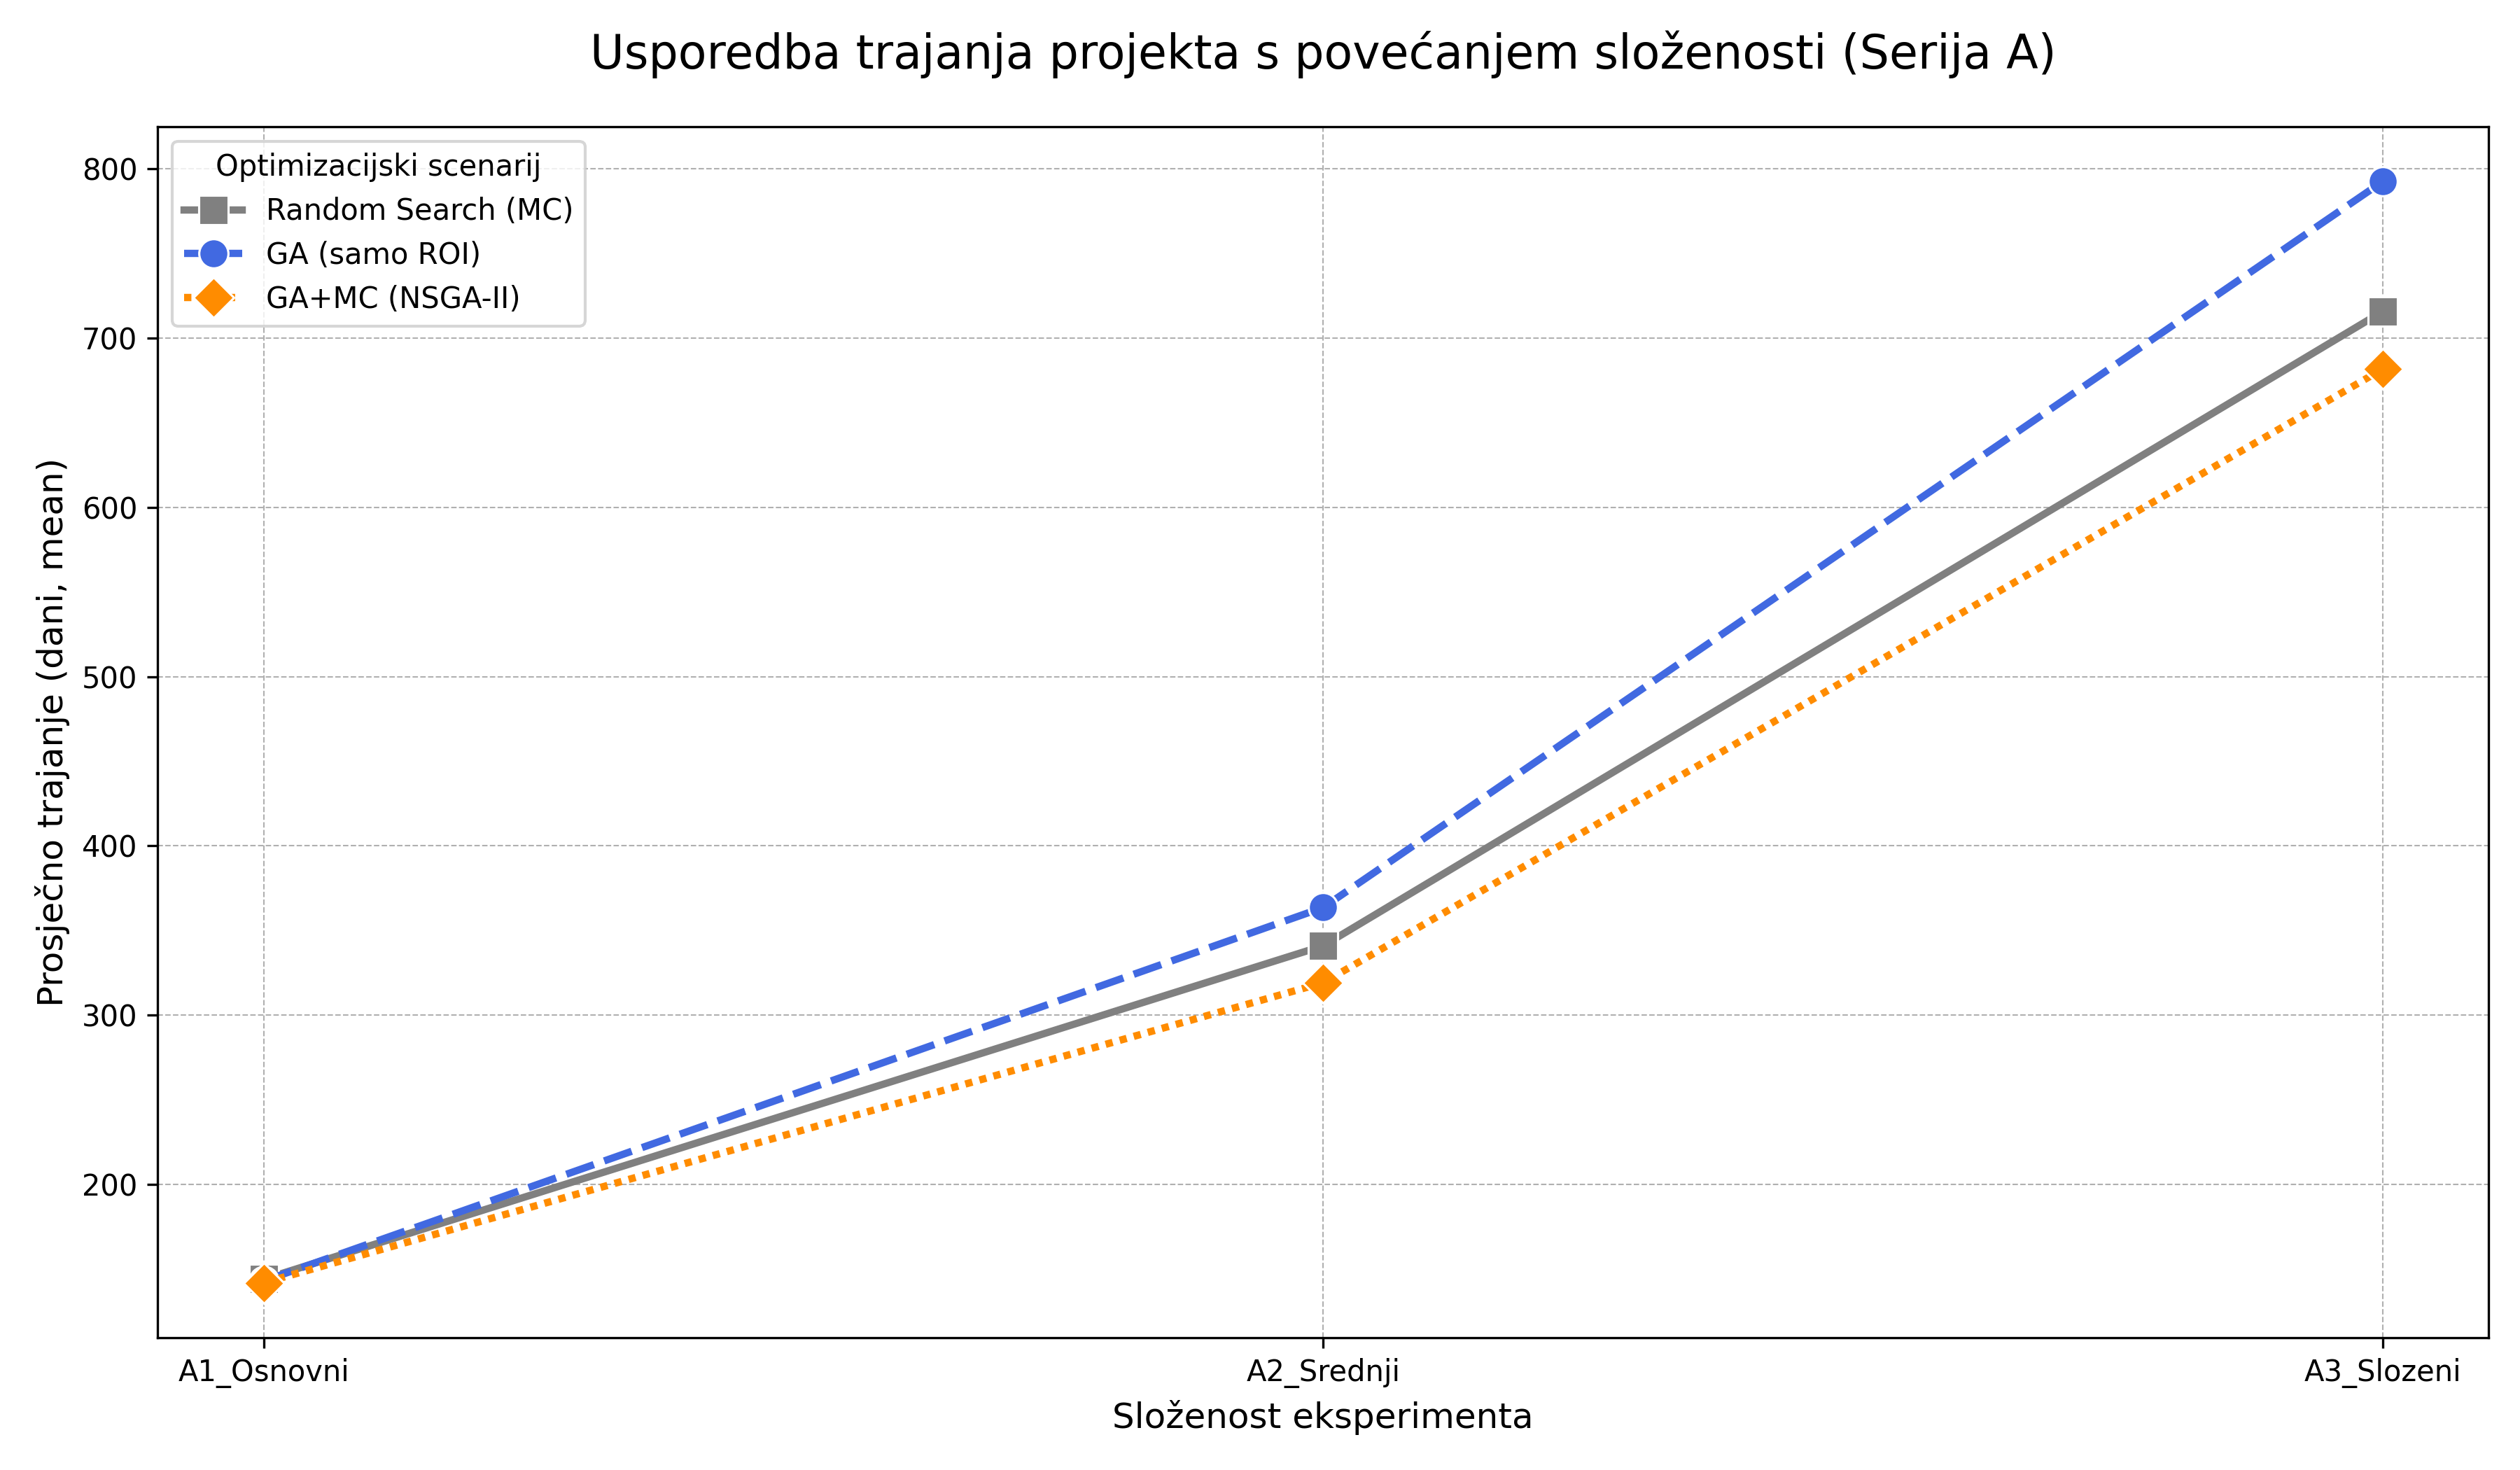
\includegraphics[width=\textwidth]{slike/grafikoni_final/A_skalabilnost_trajanje.png}
        \caption{Usporedba prosječnog trajanja.}
    \end{subfigure}
    \caption{Grafički prikaz rezultata Serije A: Usporedba modela u uvjetima rastuće složenosti.}
    \label{fig:a_skalabilnost}
\end{figure}

\textbf{Analiza Utjecaja Ograničenja (Serija B)}
Slika~\ref{fig:budzet_roi} ilustrira ponašanje modela pod različitim proračunskim pritiskom. Najvažniji nalaz dolazi iz eksperimenta s restriktivnim budžetom (B1), gdje GA+MC (NSGA-II) pokazuje iznimnu krhkost, ne uspijevajući pronaći valjano rješenje u 50\% pokretanja. S druge strane, jednostavniji GA (samo ROI) pokazuje se vrlo robusnim. Ovo ukazuje da složenost više-kriterijske pretrage može biti nedostatak u ekstremno suženim prostorima rješenja. U uvjetima labavog budžeta (B3), svi modeli rade očekivano dobro, potvrđujući hipotezu H3.

\begin{figure}[H]
    \centering
    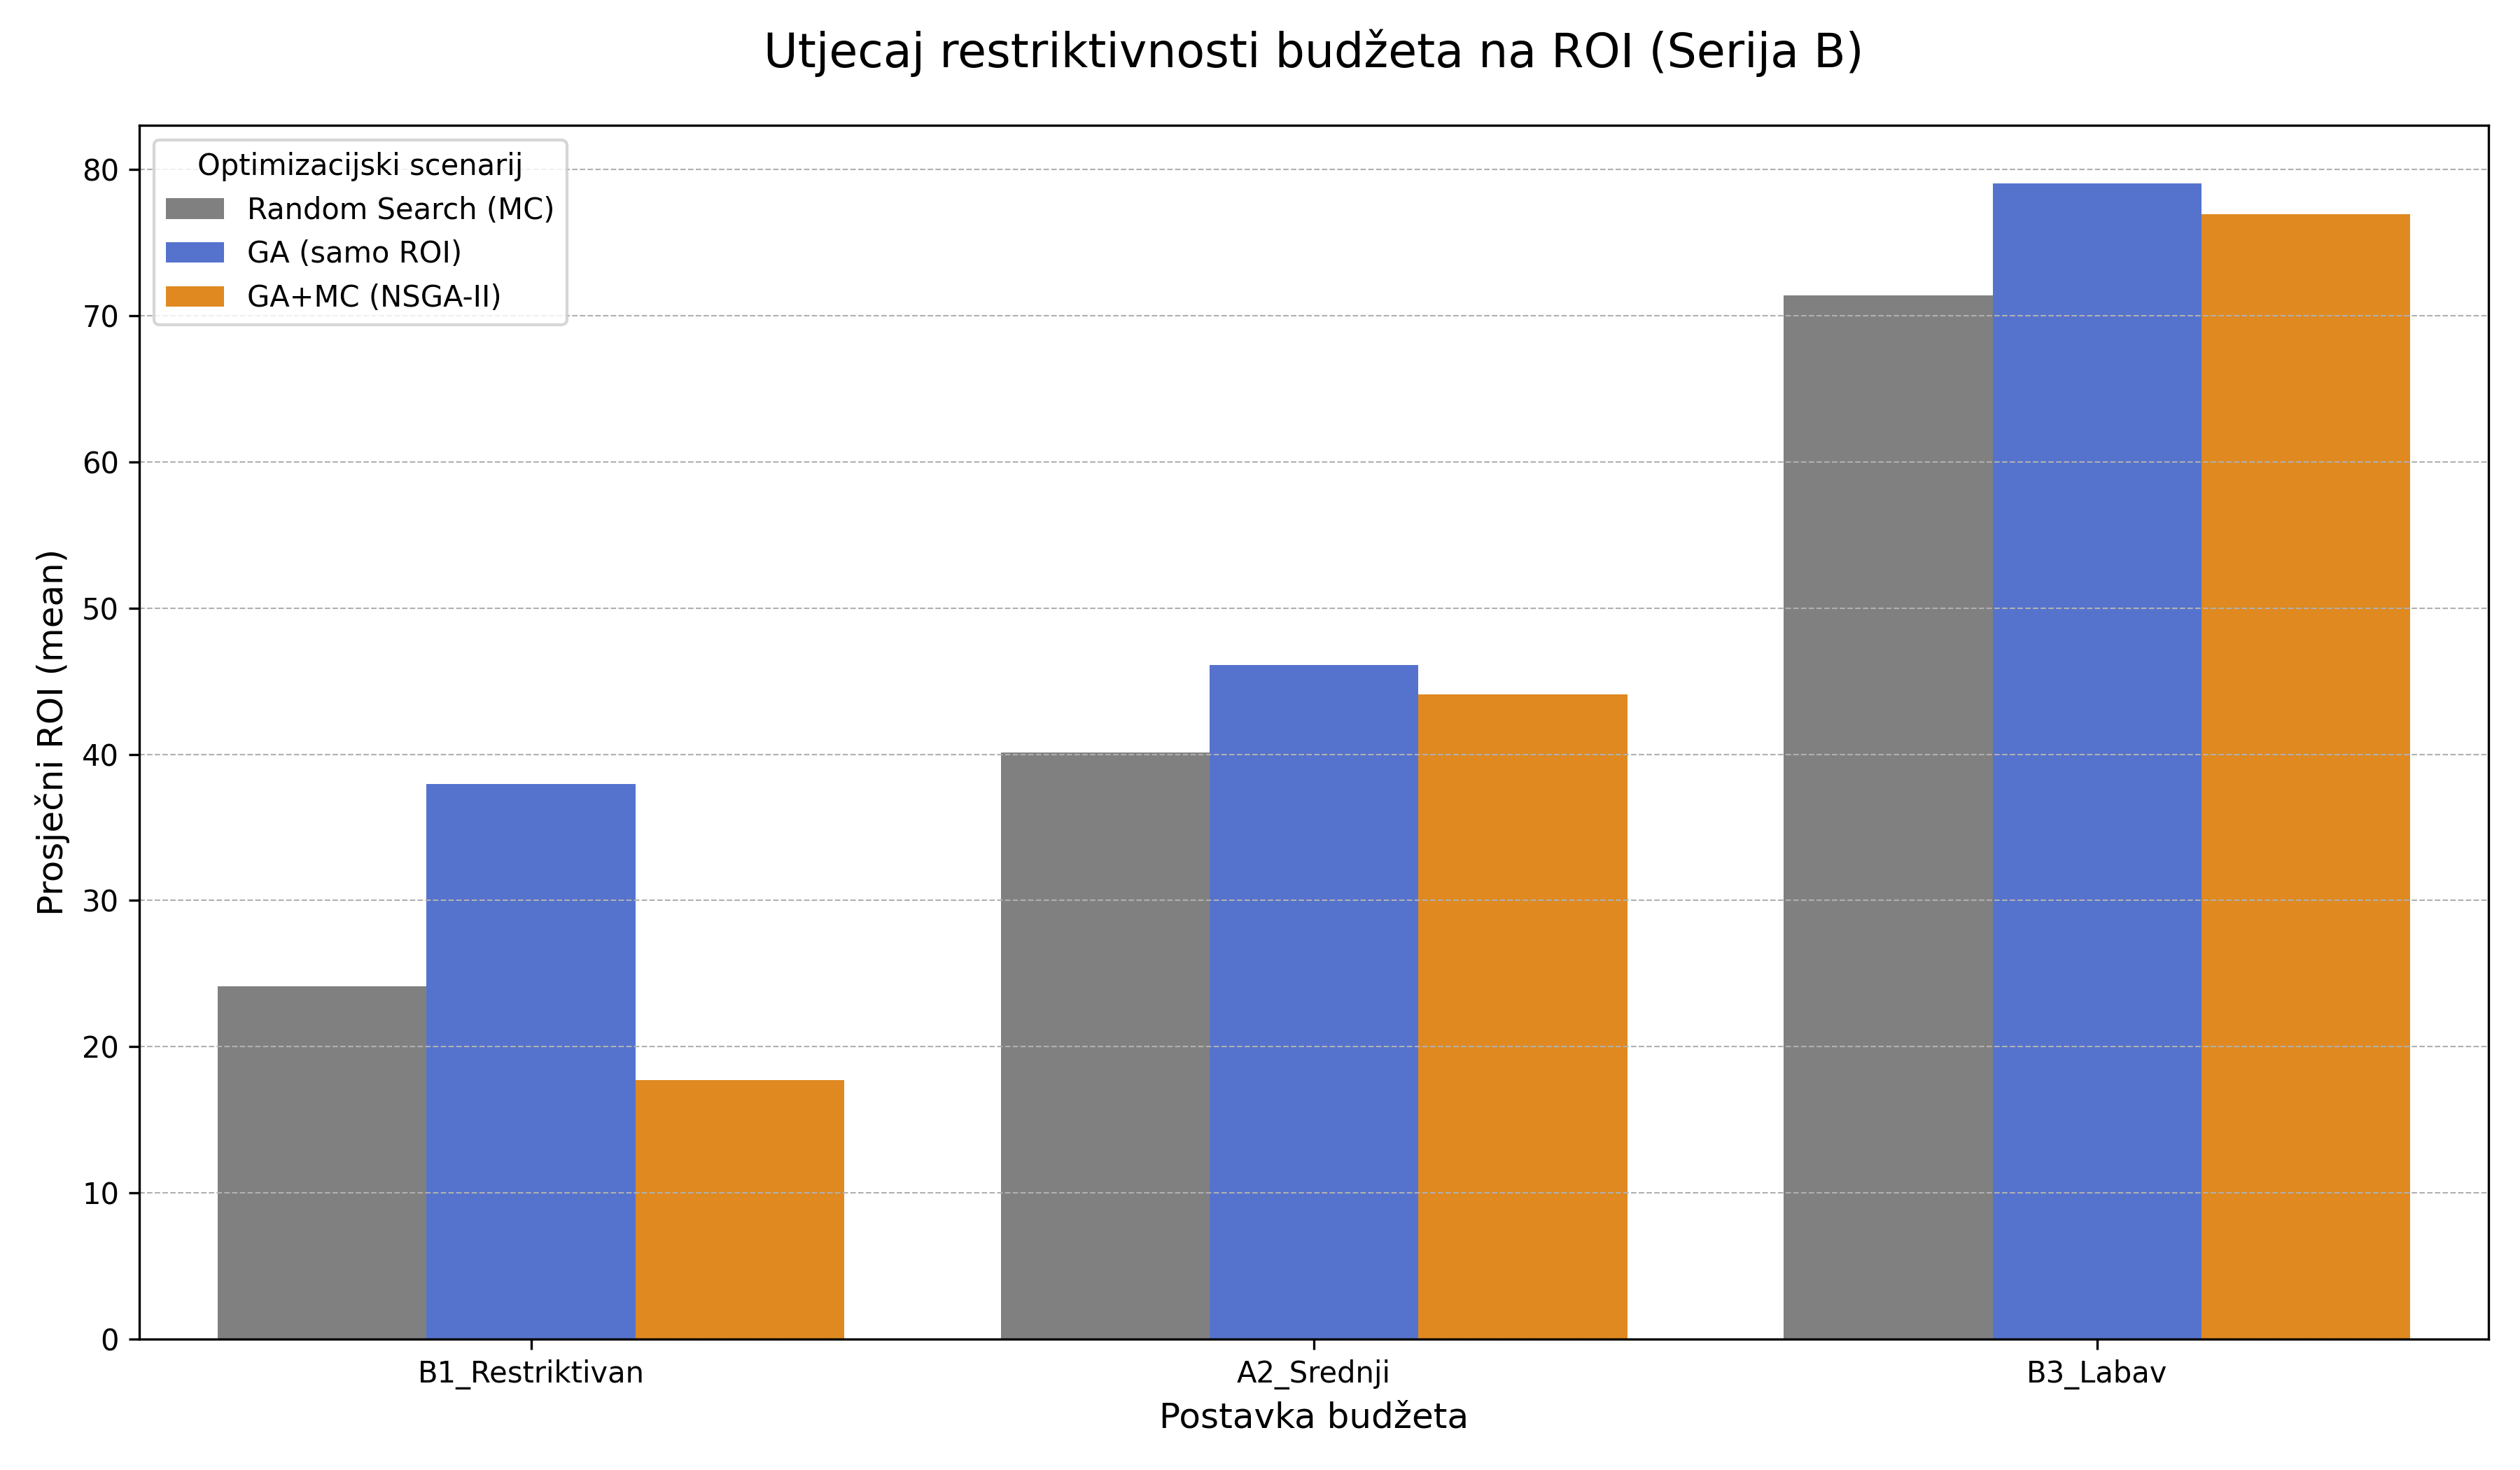
\includegraphics[width=0.8\textwidth]{slike/grafikoni_final/B_budzet_roi.png}
    \caption{Usporedba prosječnog ROI-a modela pod različitim proračunskim ograničenjima (Serija B).}
    \label{fig:budzet_roi}
\end{figure}

\textbf{Analiza Stabilnosti i Pouzdanosti}
Grafikoni na Slici~\ref{fig:stabilnost} prikazuju standardnu devijaciju kao mjeru konzistentnosti. Izvan scenarija B1 gdje je doživio neuspjeh, GA+MC (NSGA-II) model pokazuje usporedivu ili nižu devijaciju trajanja u odnosu na klasični GA. To implicira da rješenja koja nudi nisu samo u prosjeku brža, već su i pouzdanija.

\begin{figure}[H]
    \centering
    \begin{subfigure}[b]{0.48\textwidth}
        \centering
        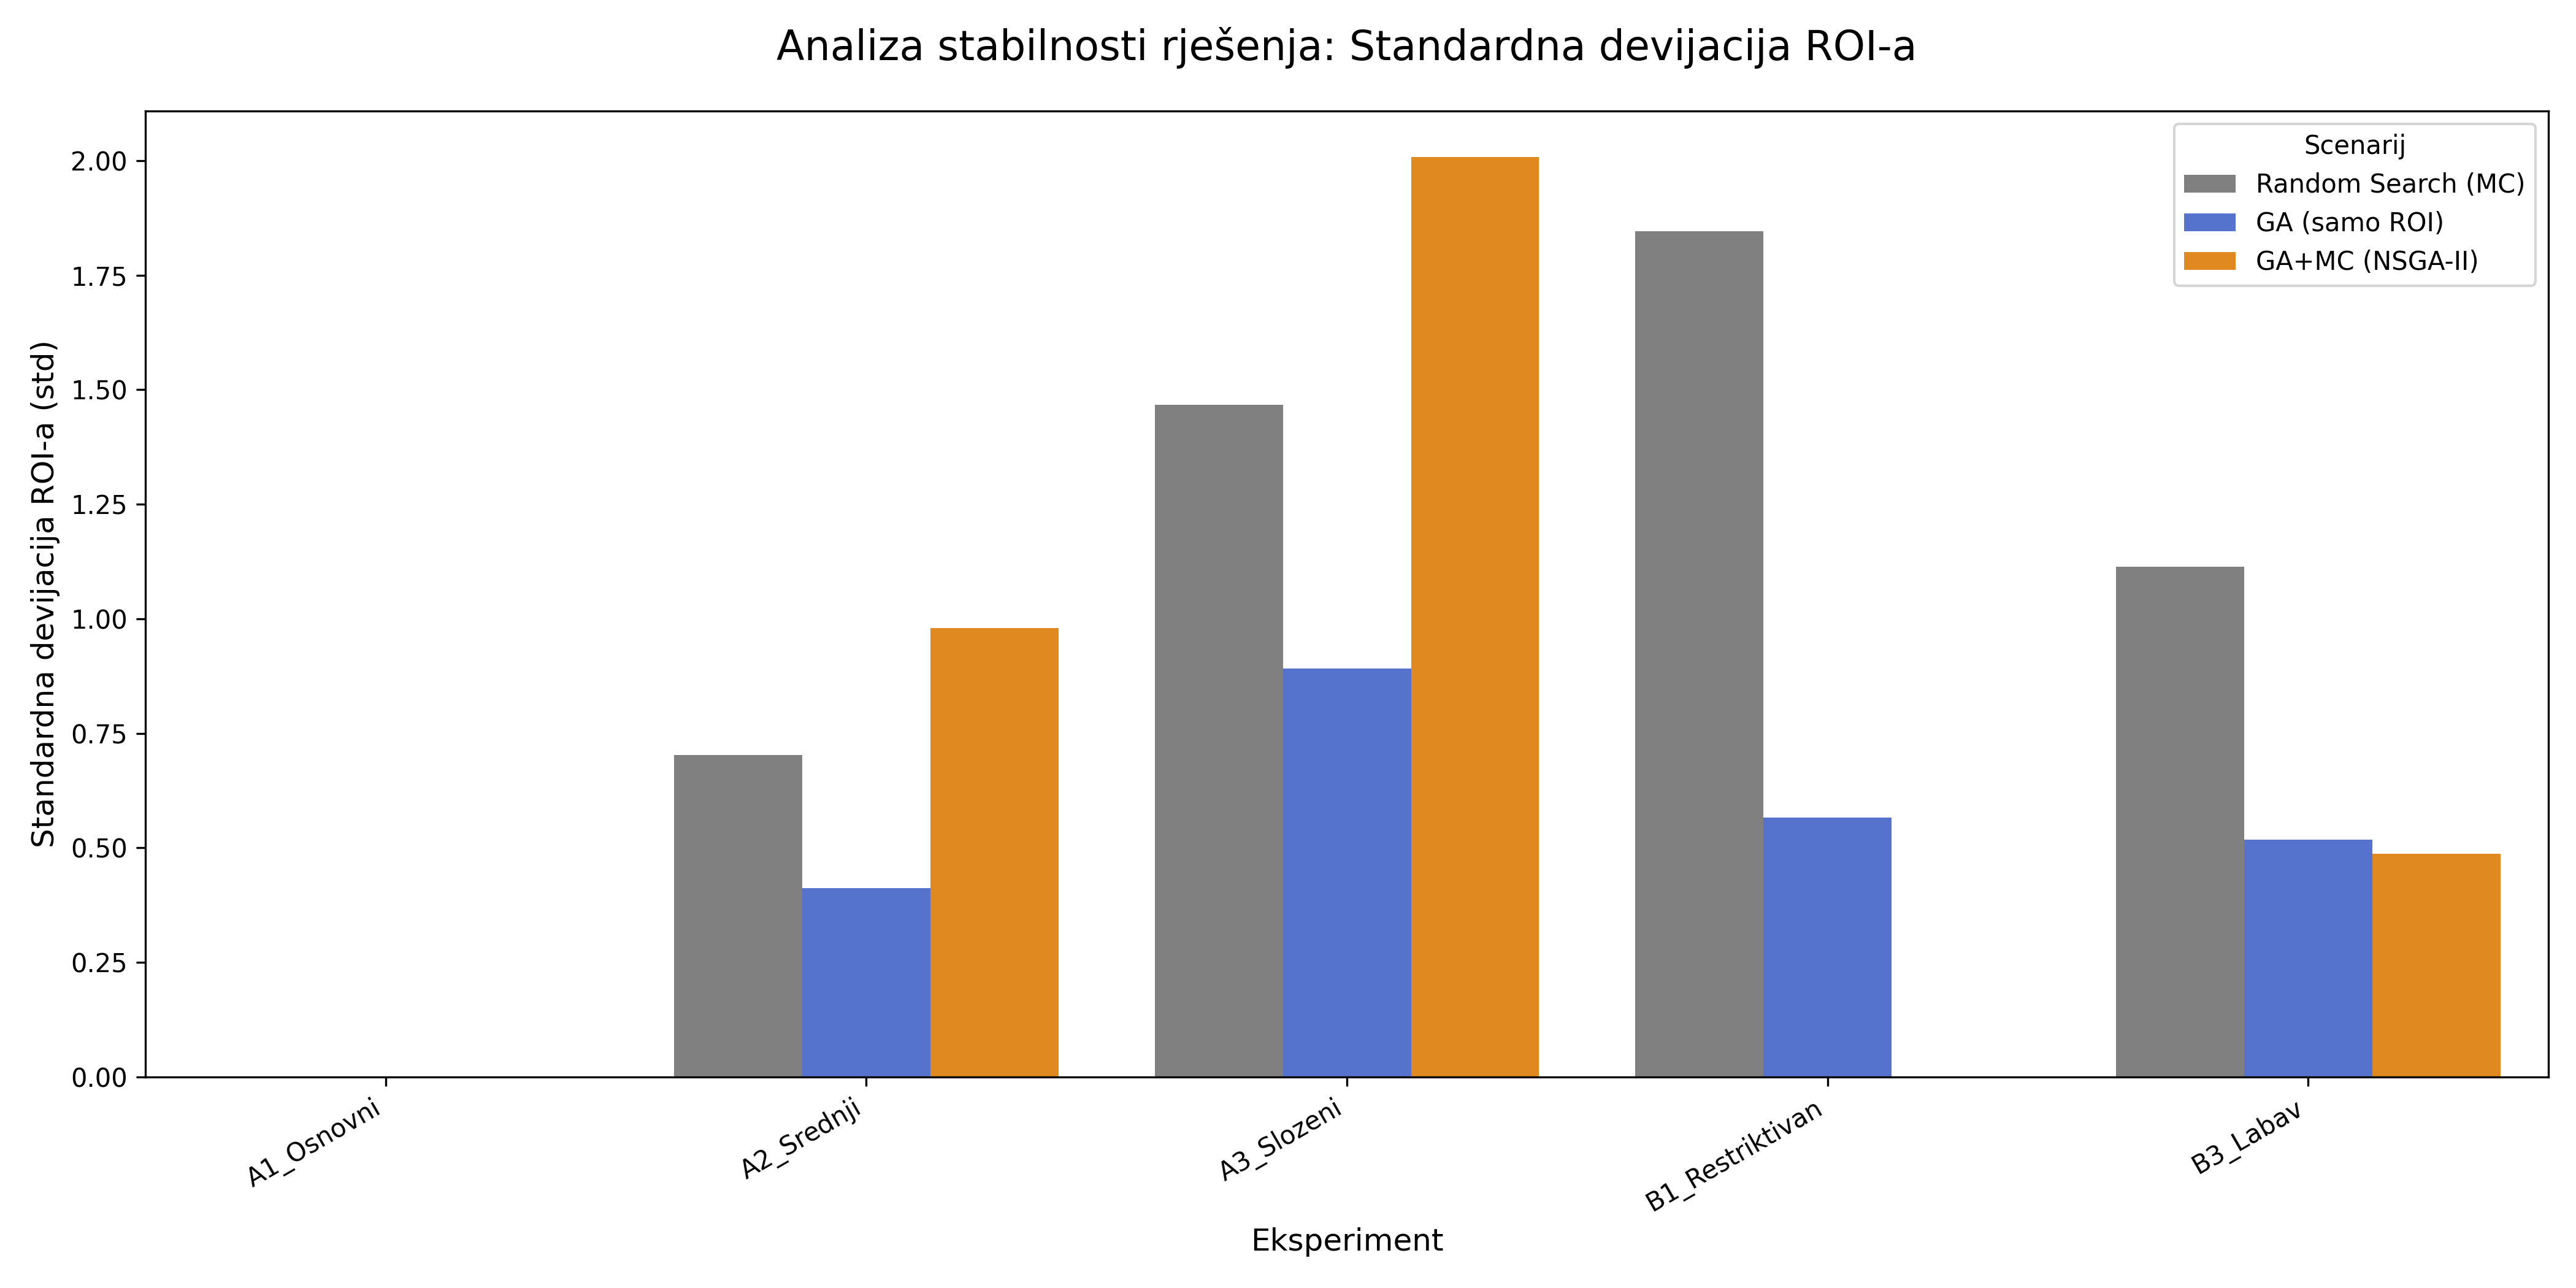
\includegraphics[width=\textwidth]{slike/grafikoni_final/C_stabilnost_roi.png}
        \caption{Stabilnost ROI-a.}
    \end{subfigure}
    \hfill
    \begin{subfigure}[b]{0.48\textwidth}
        \centering
        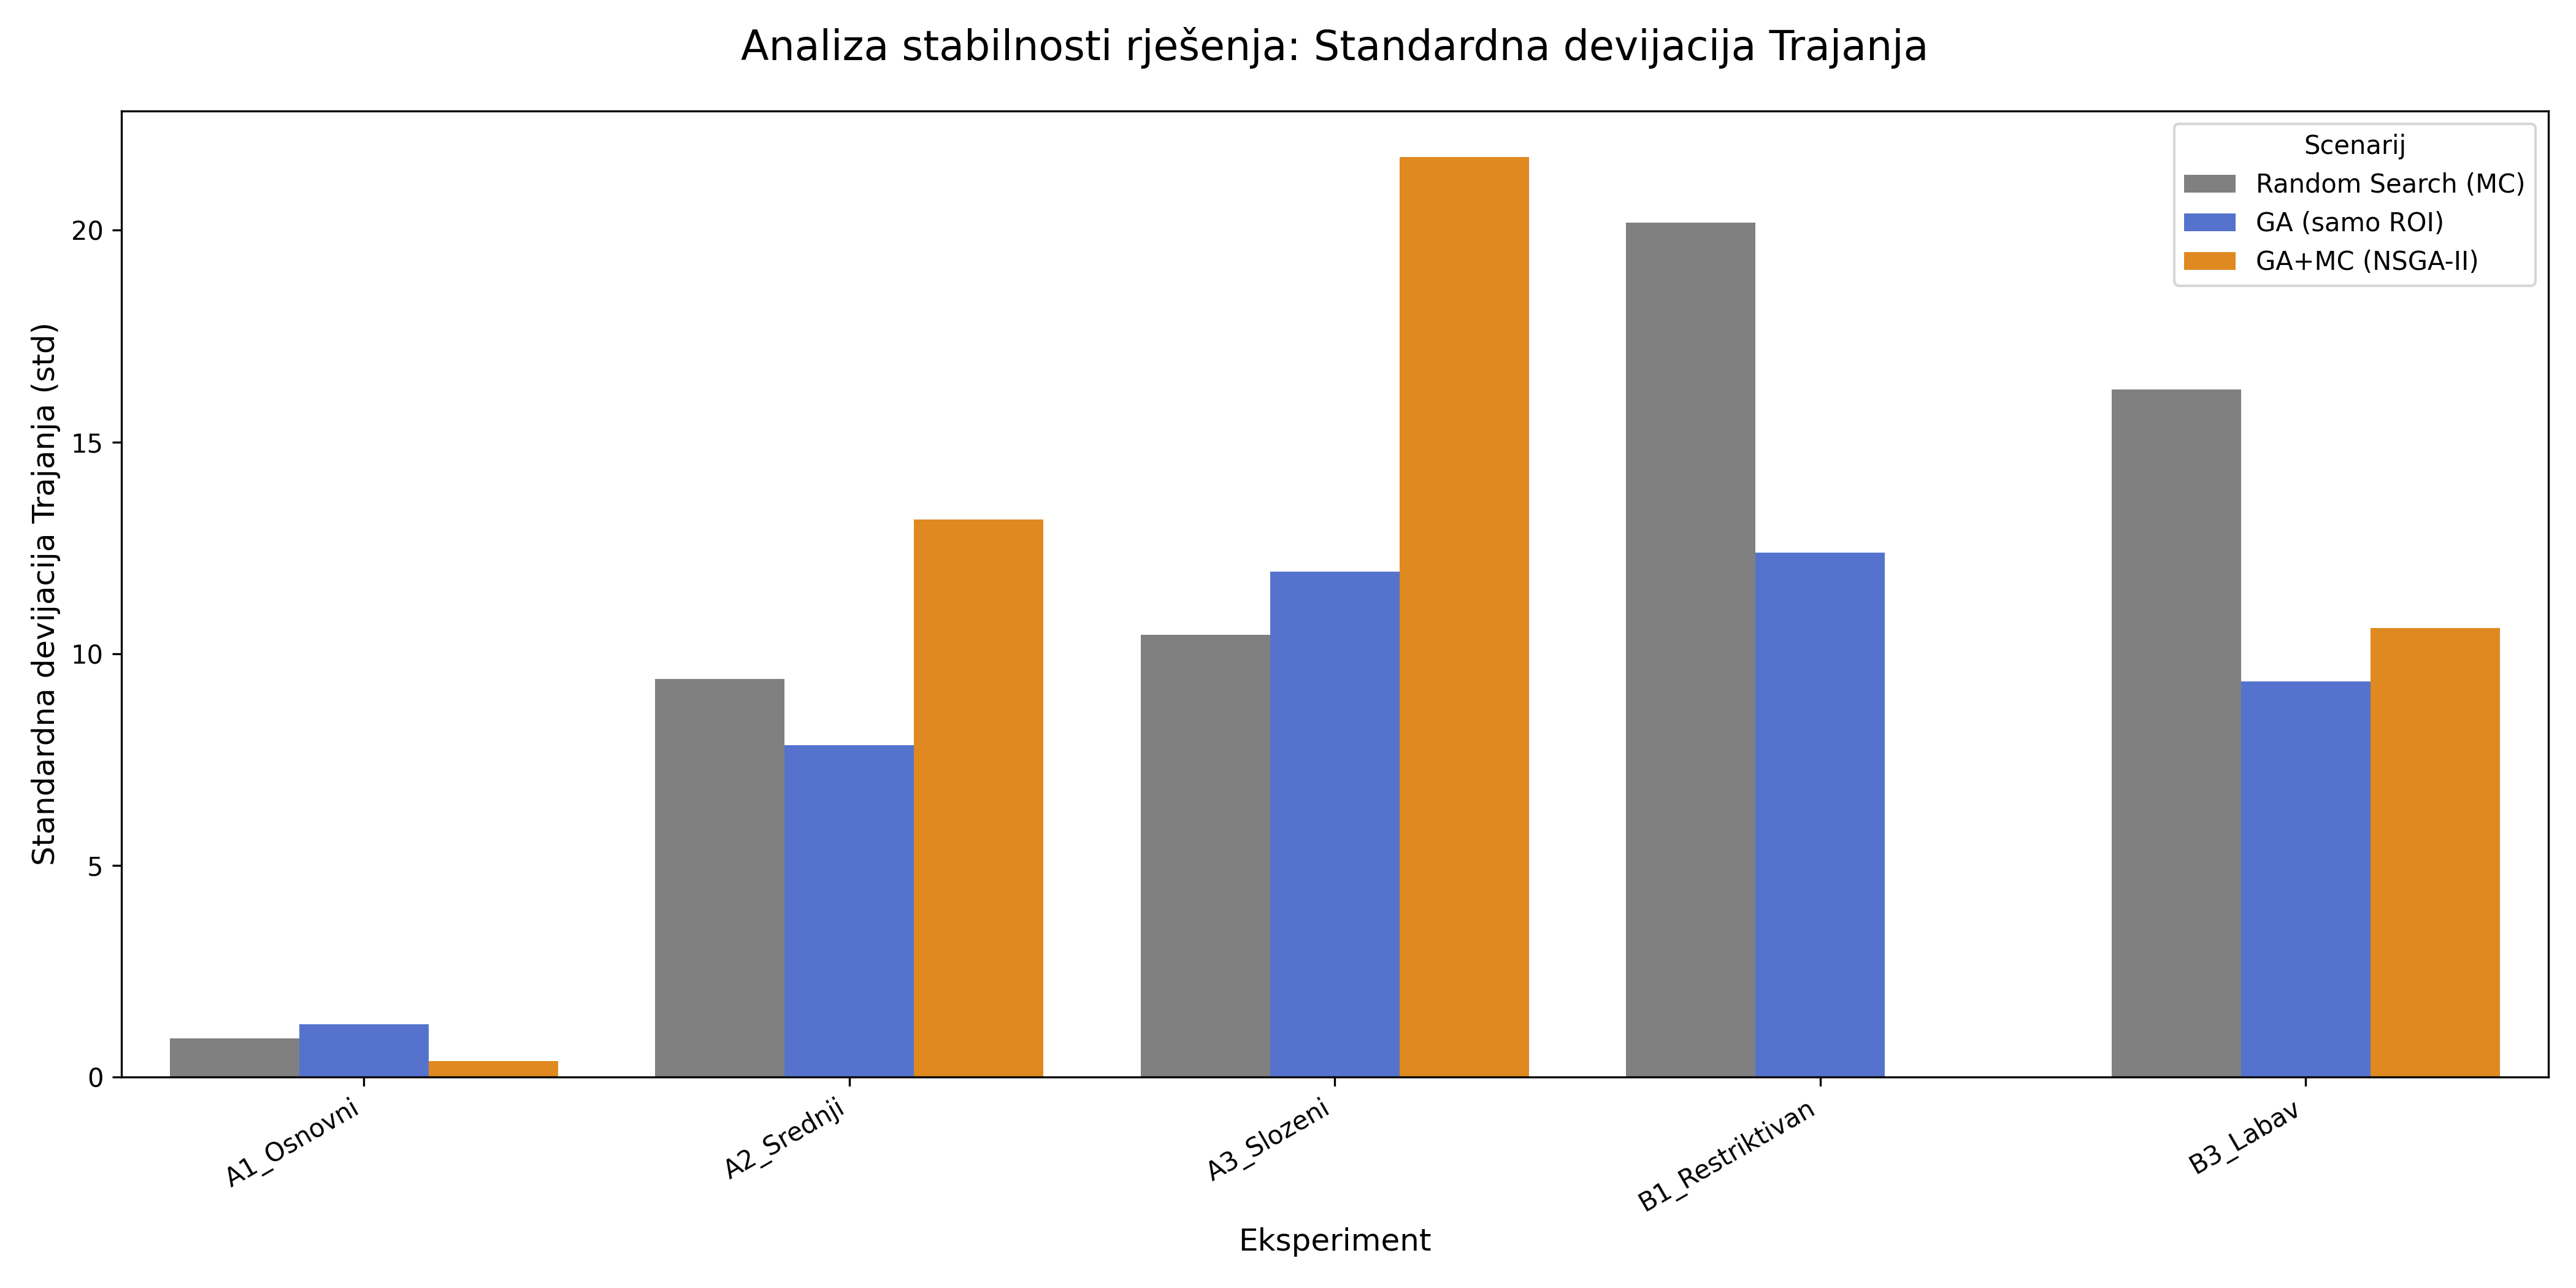
\includegraphics[width=\textwidth]{slike/grafikoni_final/C_stabilnost_trajanje.png}
        \caption{Stabilnost trajanja.}
    \end{subfigure}
    \caption{Grafički prikaz stabilnosti rješenja: Standardna devijacija za ROI i Trajanje.}
    \label{fig:stabilnost}
\end{figure}

\textbf{Dubinska analiza kompromisa: Paretov front}
Raspršeni dijagram na Slici~\ref{fig:pareto_front} pruža dubinski uvid u srž više-kriterijske optimizacije. On prikazuje Paretov front dobiven iz jednog pokretanja GA+MC (NSGA-II) modela na najsloženijem problemu (A3). Svaka točka na grafikonu predstavlja jedno optimalno, ne-dominirano rješenje i ilustrira temeljni kompromis (\emph{trade-off}) između profitabilnosti (Y-os) i rizika trajanja (X-os). Paretov front stoga ne nudi jedno "točno" rješenje, već služi kao strateški alat za donošenje odluka.

\begin{figure}[H]
    \centering
    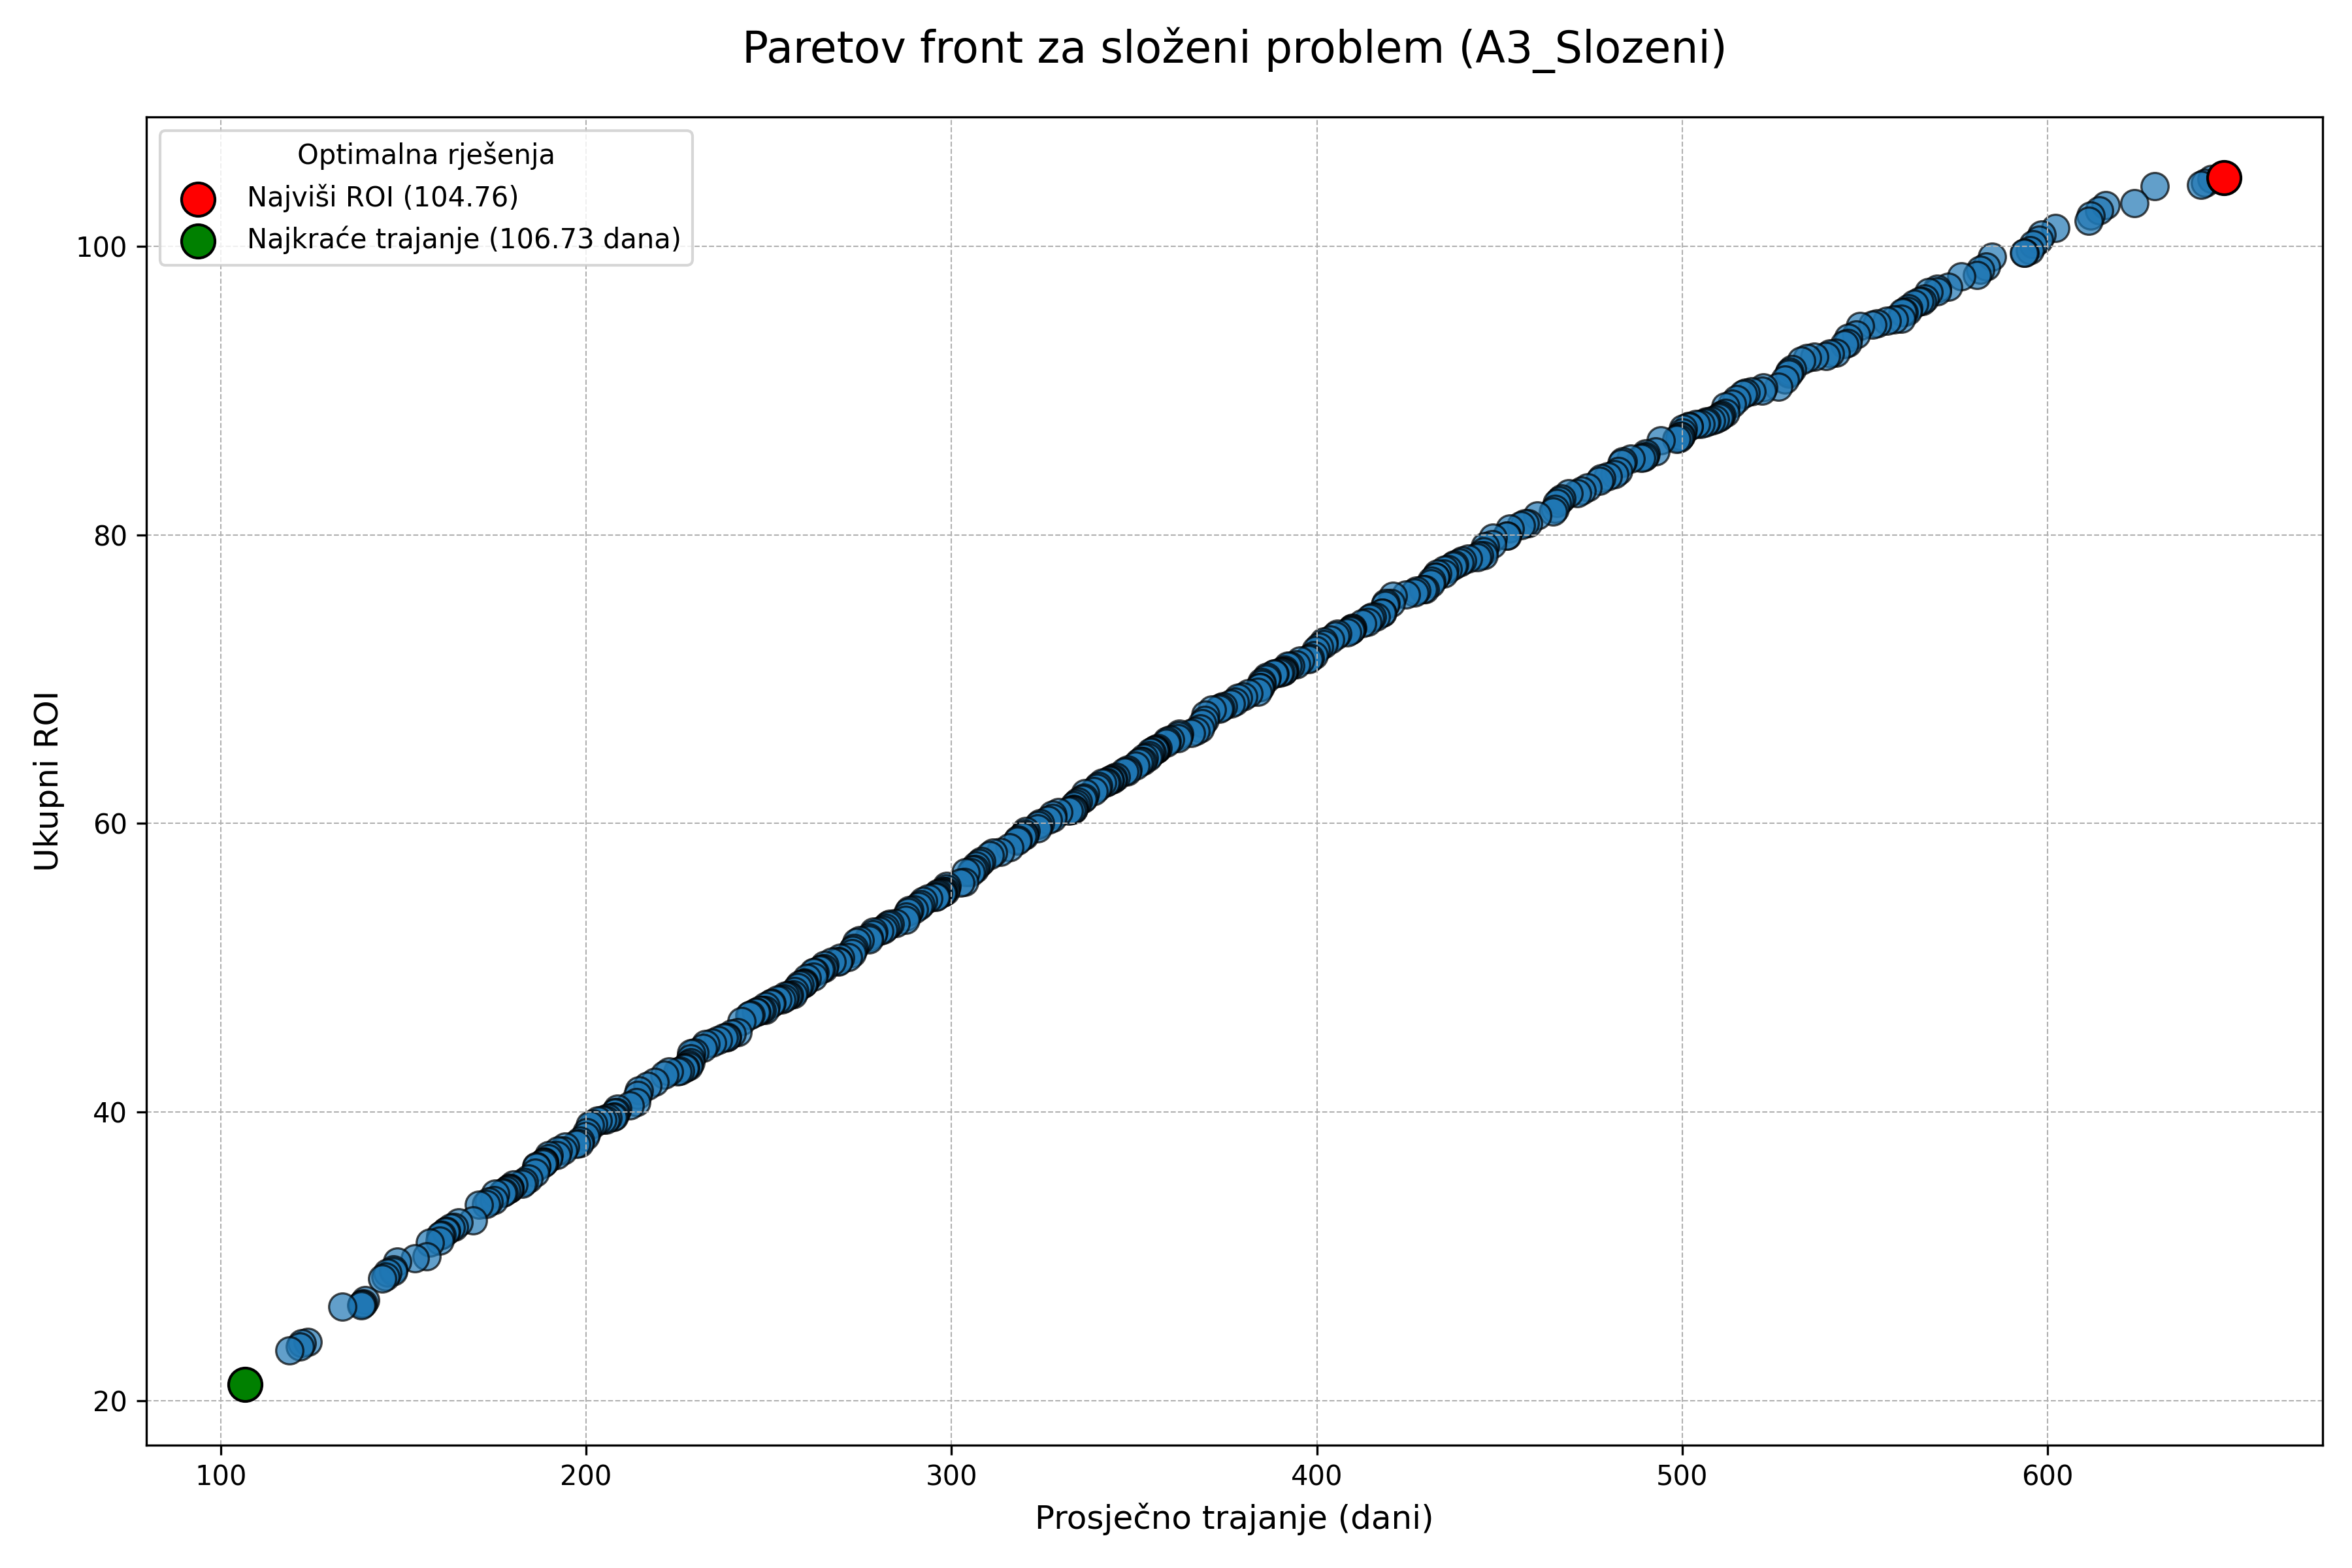
\includegraphics[width=0.9\textwidth]{slike/grafikoni_final/D_pareto_front_scatter.png}
    \caption{Paretov front za složeni problem (A3), koji prikazuje kompromis između ROI-a i trajanja.}
    \label{fig:pareto_front}
\end{figure}

\subsection{Sinteza i interpretacija glavnih nalaza}
Provedeni eksperimenti omogućuju donošenje cjelovitih zaključaka o svakom modelu. Random Search (MC) se pokazao korisnim isključivo kao početna točka na jednostavnim problemima, ali je potpuno neadekvatan kao ozbiljan optimizacijski alat za probleme realne veličine. GA (samo ROI) je izuzetno snažan i robustan "profitni maksimizator", idealan u situacijama gdje je financijska dobit jedini kriterij. Konačno, GA+MC (NSGA-II) je sofisticirani "upravitelj rizikom", čija najveća vrijednost leži u pružanju strateških opcija koje balansiraju profit i rizik. Iako je superioran u standardnim i složenim uvjetima, njegova složenost ga čini osjetljivim u okruženjima s ekstremno restriktivnim ograničenjima.

Konačan izbor modela stoga ovisi o strateškim prioritetima projektnog ureda. Za maksimalan profit, klasični GA je pobjednik. Za uravnoteženo i rizikom informirano donošenje odluka, hibridni GA+MC je superioran, uz nužan oprez pri primjeni u vrlo ograničenim uvjetima.


Nakon detaljne analize pojedinačnih serija eksperimenata, mogu se sintetizirati ključni nalazi koji zajedno oslikavaju cjelovitu sliku o performansama, prednostima i nedostacima svakog od testiranih optimizacijskih modela. Interpretacija ovih nalaza pruža direktne odgovore na postavljene istraživačke hipoteze.

Potvrda superiornosti genetskih algoritama (H1):
Prvi i najjasniji zaključak jest da je hipoteza o skalabilnosti (H1) u potpunosti potvrđena. Iako je Random Search metoda, zbog velikog broja evaluacija, uspijevala pronaći valjana rješenja, njezina učinkovitost nije pratila eksponencijalni rast složenosti problema. S druge strane, oba genetska algoritma pokazala su sposobnost inteligentno vođene pretrage, konzistentno pronalazeći značajno superiornija rješenja. Za projektnog menadžera, praktična implikacija je nedvosmislena: za bilo koji netrivijalan problem odabira portfelja, primjena metaheurističkih metoda poput genetskih algoritama nije samo poboljšanje, već nužnost za postizanje konkurentnih rezultata.

Kvantifikacija kompromisa između profita i rizika (H2):
Središnji nalaz istraživanja proizašao je iz usporedbe dvaju genetskih algoritama. Model GA (samo ROI) se dokazao kao iznimno učinkovit "profitni maksimizator", konzistentno pronalazeći rješenja s najvišim mogućim povratom na investiciju. Međutim, bio je potpuno "slijep" na rizik trajanja, često birajući portfelje s dugim i nepredvidljivim vremenom izvođenja.

Tu do izražaja dolazi ključni doprinos hibridnog GA+MC (NSGA-II) modela. Njegova svrha nije bila nadmašiti klasični GA u jednoj dimenziji (ROI), već otkriti i kvantificirati sam kompromis između profitabilnosti i rizika, čime je potvrđena hipoteza H2. Kao što rezultati i Paretov front (Slika~\ref{fig:pareto_front}) pokazuju, hibridni model omogućuje donošenje strateške odluke. On kvantificira "cijenu" smanjenja rizika, pokazujući, primjerice, da se za 5-10% niži ROI može dobiti portfelj koji je 15-25% brži i, što je još važnije, statistički pouzdaniji. Za donositelja odluka, ovo transformira optimizacijski problem iz potrage za jednim brojem u sofisticirani alat za strateško planiranje.

Otkriće o robusnosti i krhkosti modela (H3):
Konačno, analiza utjecaja ograničenja (Serija B) potvrdila je hipotezu H3 i dovela do najdubljeg i pomalo neočekivanog zaključka. Dok je klasični GA (samo ROI) pokazao iznimnu robusnost, pronalazeći dobra rješenja čak i pod vrlo restriktivnim budžetom, napredni GA+MC (NSGA-II) model pokazao je neočekivanu krhkost. Njegov složeni, više-kriterijski mehanizam pretrage, koji briljira u velikim i otvorenim prostorima rješenja, postao je njegova slabost u ekstremno suženom prostoru valjanih opcija, što je dovelo do čestih neuspjeha.

Ovaj nalaz nosi ključnu praktičnu poruku: tehnološki najnapredniji alat nije uvijek najbolji alat za svaku situaciju. U kriznim scenarijima s ekstremno ograničenim resursima, jednostavniji i fokusiraniji pristup može biti pouzdaniji.

Za lakši pregled, konačna ocjena svakog modela sažeta je u Tablici~\ref{tab:sinteza_modela}.


\begin{table}[H]
\centering
\caption{Sintetička usporedba evaluiranih modela.}
\label{tab:sinteza_modela}
\resizebox{\textwidth}{!}{
\begin{tabular}{|l|l|l|}
\hline
\textbf{Model} & \textbf{Najbolji za...} & \textbf{Ključna ograničenja} \\
\hline
\textbf{Random Search (MC)} & Postavljanje osnovne linije (baseline) na jednostavnim problemima. & Potpuno neefikasan i nepouzdan na složenim problemima. \\
\hline
\textbf{GA (samo ROI)} & Scenarije gdje je maksimizacija profita jedini i isključivi cilj. & Zanemaruje rizik trajanja; može predložiti vrlo duge projekte. \\
\hline
\textbf{GA+MC (NSGA-II)} & Strateško odlučivanje; balansiranje između profita i rizika. & Računalno zahtjevan; nepouzdan u ekstremno restriktivnim uvjetima. \\
\hline
\end{tabular}
}
\end{table}
Konačan izbor modela stoga ovisi o strateškim prioritetima projektnog ureda. Za maksimalan profit, klasični GA je pobjednik. Za uravnoteženo i rizikom informirano donošenje odluka, hibridni GA+MC je superioran, uz nužan oprez pri primjeni u vrlo ograničenim uvjetima.

\newpage

\section{Zaključak}

U ovom diplomskom radu predstavili smo kompleksan pristup optimizaciji raspodjele projektnih aktivnosti koristeći kombinaciju genetskih algoritama i Monte Carlo simulacije. Cilj je bio razviti model koji uzima u obzir nesigurnost u trajanju, troškovima i vrijednosti zadataka, te u okviru zadanih ograničenja vremena, budžeta i raspoloživih resursa maksimizira ukupnu vrijednost projekta.

Kroz detaljnu analizu problematike i pregled postojeće literature, identificirali smo ključne izazove u upravljanju projektima, posebice u segmentu neizvjesnosti i složenosti optimizacije. Implementacijom metaheurističkih metoda, u ovom slučaju genetskih algoritama \cite{Goldberg1989, Mitchell1998}, omogućili smo efikasno pretraživanje velikog prostora rješenja, dok je Monte Carlo simulacija služila za kvantitativno modeliranje rizika i nesigurnosti \cite{Miller2009, Avlijas2008}, dajući time realističniju procjenu performansi optimizacijskog rješenja.

Praktična implementacija rezultirala je modelom koji omogućuje donošenje informiranih odluka u planiranju i upravljanju projektima, pružajući projektnim menadžerima alate za bolje usklađivanje ciljeva i ograničenja. Pokazalo se da je kombinacija ovih metoda učinkovita u pronalasku balansiranih rješenja koja maksimiziraju povrat ulaganja, uz minimizaciju rizika od prekoračenja budžeta ili rokova.

Iako su postignuti rezultati zadovoljavajući, postoje brojna područja za buduća istraživanja i unaprjeđenja, među kojima izdvajamo:
\begin{itemize}
    \item Proširenje modela na dinamičke uvjete projekata koji se mijenjaju tijekom vremena, uključujući nepredvidive vanjske utjecaje.
    \item Integracija dodatnih metaheurističkih i hibridnih algoritama, poput algoritama rojčaste inteligencije ili simuliranog kaljenja, radi poboljšanja kvalitete rješenja \cite{Gandomi2013}.
    \item Primjena tehnika strojnog učenja za preciznije predviđanje distribucija nesigurnosti i automatsku adaptaciju parametara optimizacije.
    \item Razvoj softverskih alata s intuitivnim korisničkim sučeljem za praktičnu primjenu predloženih metoda u realnim projektnim okruženjima.
\end{itemize}

Zaključno, ovaj rad potvrđuje važnost primjene naprednih algoritamskih rješenja u upravljanju projektima, posebno u uvjetima nesigurnosti, te doprinosi boljem razumijevanju i praktičnoj primjeni optimizacijskih i simulacijskih metoda u području projektne ekonomike i menadžmenta. Kao što ističe Kerzner \cite{Kerzner2017}, učinkovito upravljanje projektima u suvremenom okruženju zahtijeva kombinaciju tradicionalnih i naprednih pristupa, a naš model pruža značajan doprinos u tom smjeru.



\newpage

\bibliographystyle{unsrt}
\bibliography{literatura}
\newpage

%Automatski generira listu svih slika
\listoffigures
\newpage

%Automatski generira listu svih tablica
\listoftables
\newpage

%Automatski generira listu svih isječaka kodova
\phantomsection
\addcontentsline{toc}{section}{Popis kodova}
\lstlistoflistings
\newpage

\textbf{Rezultati svih provedenih eksperimenata}

\textbf{Eksperiment: \texttt{A1\_Osnovni}}
Korištena konfiguracija: \texttt{'RUNS': 10, 'NUM\_SIMULATIONS': 100, 'name': 'A1\_Osnovni', 'NUM\_ACTIVITIES': 10, 'BUDGET': 1000, 'POP\_SIZE': 100, 'NGEN': 40, 'CX\_PB': 0.7, 'MUT\_PB': 0.2}

\textbf{Pokrećem scenarij: Random Search (MC) (10 puta)}
\begin{itemize}
    \item Run 1/10: ROI=17.14, Trajanje=143.50
    \item Run 2/10: ROI=17.14, Trajanje=145.12
    \item Run 3/10: ROI=17.14, Trajanje=144.16
    \item Run 4/10: ROI=17.14, Trajanje=144.53
    \item Run 5/10: ROI=17.14, Trajanje=144.41
    \item Run 6/10: ROI=17.14, Trajanje=144.18
    \item Run 7/10: ROI=17.14, Trajanje=143.92
    \item Run 8/10: ROI=17.14, Trajanje=143.16
    \item Run 9/10: ROI=17.14, Trajanje=145.95
    \item Run 10/10: ROI=17.14, Trajanje=142.58
\end{itemize}

\textbf{Pokrećem scenarij: GA (samo ROI) (10 puta)}
\begin{itemize}
    \item Run 1/10: ROI=17.14, Trajanje=144.94
    \item Run 2/10: ROI=17.14, Trajanje=143.69
    \item Run 3/10: ROI=17.14, Trajanje=142.27
    \item Run 4/10: ROI=17.14, Trajanje=140.85
    \item Run 5/10: ROI=17.14, Trajanje=143.14
    \item Run 6/10: ROI=17.14, Trajanje=143.63
    \item Run 7/10: ROI=17.14, Trajanje=144.16
    \item Run 8/10: ROI=17.14, Trajanje=142.14
    \item Run 9/10: ROI=17.14, Trajanje=144.43
    \item Run 10/10: ROI=17.14, Trajanje=141.78
\end{itemize}

\textbf{Pokrećem scenarij: GA+MC (NSGA-II) (10 puta)}
\begin{itemize}
    \item Run 1/10: ROI=17.14, Trajanje=141.92
    \item Run 2/10: ROI=17.14, Trajanje=142.10
    \item Run 3/10: ROI=17.14, Trajanje=142.36
    \item Run 4/10: ROI=17.14, Trajanje=141.75
    \item Run 5/10: ROI=17.14, Trajanje=142.51
    \item Run 6/10: ROI=17.14, Trajanje=141.44
    \item Run 7/10: ROI=17.14, Trajanje=142.60
    \item Run 8/10: ROI=17.14, Trajanje=141.54
    \item Run 9/10: ROI=17.14, Trajanje=141.90
    \item Run 10/10: ROI=17.14, Trajanje=141.92
\end{itemize}

\textbf{Eksperiment: \texttt{A2\_Srednji}}
Korištena konfiguracija: \texttt{'RUNS': 10, 'NUM\_SIMULATIONS': 100, 'name': 'A2\_Srednji', 'NUM\_ACTIVITIES': 50, 'BUDGET': 2500, 'POP\_SIZE': 200, 'NGEN': 150, 'CX\_PB': 0.7, 'MUT\_PB': 0.2}

\textbf{Pokrećem scenarij: Random Search (MC) (10 puta)}
\begin{itemize}
    \item Run 1/10: ROI=40.40, Trajanje=337.68
    \item Run 2/10: ROI=40.66, Trajanje=338.59
    \item Run 3/10: ROI=41.85, Trajanje=365.09
    \item Run 4/10: ROI=40.12, Trajanje=335.75
    \item Run 5/10: ROI=39.45, Trajanje=333.62
    \item Run 6/10: ROI=39.44, Trajanje=344.36
    \item Run 7/10: ROI=40.17, Trajanje=341.35
    \item Run 8/10: ROI=39.50, Trajanje=339.48
    \item Run 9/10: ROI=39.76, Trajanje=346.14
    \item Run 10/10: ROI=39.73, Trajanje=328.16
\end{itemize}

\textbf{Pokrećem scenarij: GA (samo ROI) (10 puta)}
\begin{itemize}
    \item Run 1/10: ROI=46.49, Trajanje=361.80
    \item Run 2/10: ROI=46.99, Trajanje=367.77
    \item Run 3/10: ROI=45.84, Trajanje=366.80
    \item Run 4/10: ROI=45.91, Trajanje=345.02
    \item Run 5/10: ROI=46.50, Trajanje=366.93
    \item Run 6/10: ROI=45.52, Trajanje=376.11
    \item Run 7/10: ROI=45.75, Trajanje=360.74
    \item Run 8/10: ROI=46.23, Trajanje=369.00
    \item Run 9/10: ROI=46.02, Trajanje=364.34
    \item Run 10/10: ROI=46.00, Trajanje=357.81
\end{itemize}

\textbf{Pokrećem scenarij: GA+MC (NSGA-II) (10 puta)}
\begin{itemize}
    \item Run 1/10: ROI=44.77, Trajanje=332.03
    \item Run 2/10: ROI=43.67, Trajanje=307.26
    \item Run 3/10: ROI=44.96, Trajanje=323.94
    \item Run 4/10: ROI=43.70, Trajanje=316.31
    \item Run 5/10: ROI=43.74, Trajanje=306.20
    \item Run 6/10: ROI=44.76, Trajanje=324.82
    \item Run 7/10: ROI=45.73, Trajanje=345.46
    \item Run 8/10: ROI=42.25, Trajanje=297.04
    \item Run 9/10: ROI=42.96, Trajanje=316.77
    \item Run 10/10: ROI=44.45, Trajanje=322.27
\end{itemize}

\textbf{Eksperiment: \texttt{A3\_Slozeni}}
Korištena konfiguracija: \texttt{'RUNS': 10, 'NUM\_SIMULATIONS': 100, 'name': 'A3\_Slozeni', 'NUM\_ACTIVITIES': 100, 'BUDGET': 5000, 'POP\_SIZE': 250, 'NGEN': 200, 'CX\_PB': 0.7, 'MUT\_PB': 0.2}

\textbf{Pokrećem scenarij: Random Search (MC) (10 puta)}
\begin{itemize}
    \item Run 1/10: ROI=95.11, Trajanje=719.00
    \item Run 2/10: ROI=95.18, Trajanje=703.35
    \item Run 3/10: ROI=95.04, Trajanje=711.90
    \item Run 4/10: ROI=93.95, Trajanje=697.17
    \item Run 5/10: ROI=95.31, Trajanje=709.34
    \item Run 6/10: ROI=94.62, Trajanje=714.26
    \item Run 7/10: ROI=99.34, Trajanje=727.76
    \item Run 8/10: ROI=96.00, Trajanje=734.40
    \item Run 9/10: ROI=97.08, Trajanje=717.74
    \item Run 10/10: ROI=96.72, Trajanje=721.11
\end{itemize}

\textbf{Pokrećem scenarij: GA (samo ROI) (10 puta)}
\begin{itemize}
    \item Run 1/10: ROI=113.18, Trajanje=805.12
    \item Run 2/10: ROI=113.49, Trajanje=807.35
    \item Run 3/10: ROI=113.75, Trajanje=790.95
    \item Run 4/10: ROI=114.73, Trajanje=789.09
    \item Run 5/10: ROI=114.54, Trajanje=788.01
    \item Run 6/10: ROI=113.37, Trajanje=775.14
    \item Run 7/10: ROI=115.26, Trajanje=775.51
    \item Run 8/10: ROI=113.56, Trajanje=812.19
    \item Run 9/10: ROI=116.09, Trajanje=792.83
    \item Run 10/10: ROI=114.27, Trajanje=786.81
\end{itemize}

\textbf{Pokrećem scenarij: GA+MC (NSGA-II) (10 puta)}
\textit{-> SPREMAM PARETOV FRONT ZA VIZUALIZACIJU...}
\begin{itemize}
    \item Run 1/10: ROI=104.76, Trajanje=648.19
    \item Run 2/10: ROI=110.63, Trajanje=709.22
    \item Run 3/10: ROI=109.97, Trajanje=688.70
    \item Run 4/10: ROI=111.60, Trajanje=703.53
    \item Run 5/10: ROI=109.98, Trajanje=675.31
    \item Run 6/10: ROI=109.66, Trajanje=680.58
    \item Run 7/10: ROI=107.36, Trajanje=673.95
    \item Run 8/10: ROI=108.42, Trajanje=667.60
    \item Run 9/10: ROI=111.22, Trajanje=715.93
    \item Run 10/10: ROI=107.35, Trajanje=652.63
\end{itemize}

\textbf{Eksperiment: \texttt{B1\_Restriktivan}}
Korištena konfiguracija: \texttt{'RUNS': 10, 'NUM\_SIMULATIONS': 100, 'name': 'B1\_Restriktivan', 'NUM\_ACTIVITIES': 50, 'BUDGET': 1500, 'POP\_SIZE': 200, 'NGEN': 150, 'CX\_PB': 0.7, 'MUT\_PB': 0.2}

\textbf{Pokrećem scenarij: Random Search (MC) (10 puta)}
\begin{itemize}
    \item Run 1/10: ROI=21.25, Trajanje=206.67
    \item Run 2/10: ROI=26.95, Trajanje=199.13
    \item Run 3/10: ROI=23.24, Trajanje=194.97
    \item Run 4/10: ROI=23.31, Trajanje=206.15
    \item Run 5/10: ROI=23.56, Trajanje=173.33
    \item Run 6/10: ROI=25.79, Trajanje=246.31
    \item Run 7/10: ROI=22.39, Trajanje=170.49
    \item Run 8/10: ROI=25.89, Trajanje=202.44
    \item Run 9/10: ROI=22.54, Trajanje=191.32
    \item Run 10/10: ROI=26.28, Trajanje=185.40
\end{itemize}

\textbf{Pokrećem scenarij: GA (samo ROI) (10 puta)}
\begin{itemize}
    \item Run 1/10: ROI=38.27, Trajanje=252.42
    \item Run 2/10: ROI=37.59, Trajanje=248.50
    \item Run 3/10: ROI=38.19, Trajanje=270.84
    \item Run 4/10: ROI=38.11, Trajanje=256.57
    \item Run 5/10: ROI=37.13, Trajanje=254.03
    \item Run 6/10: ROI=38.42, Trajanje=267.28
    \item Run 7/10: ROI=36.93, Trajanje=234.86
    \item Run 8/10: ROI=38.88, Trajanje=266.76
    \item Run 9/10: ROI=37.97, Trajanje=231.50
    \item Run 10/10: ROI=38.27, Trajanje=252.86
\end{itemize}

\textbf{Pokrećem scenarij: GA+MC (NSGA-II) (10 puta)}
\begin{itemize}
    \item Run 1/10: ROI=33.75, Trajanje=189.71
    \item Run 2/10: ROI=36.89, Trajanje=226.87
    \item Run 3/10: ROI=0.00, Trajanje=99999.00
    \item Run 4/10: ROI=35.65, Trajanje=207.29
    \item Run 5/10: ROI=0.00, Trajanje=99999.00
    \item Run 6/10: ROI=34.75, Trajanje=213.68
    \item Run 7/10: ROI=0.00, Trajanje=99999.00
    \item Run 8/10: ROI=0.00, Trajanje=99999.00
    \item Run 9/10: ROI=36.07, Trajanje=211.26
    \item Run 10/10: ROI=0.00, Trajanje=99999.00
\end{itemize}

\textbf{Eksperiment: \texttt{B3\_Labav}}
Korištena konfiguracija: \texttt{'RUNS': 10, 'NUM\_SIMULATIONS': 100, 'name': 'B3\_Labav', 'NUM\_ACTIVITIES': 50, 'BUDGET': 4000, 'POP\_SIZE': 200, 'NGEN': 150, 'CX\_PB': 0.7, 'MUT\_PB': 0.2}

\textbf{Pokrećem scenarij: Random Search (MC) (10 puta)}
\begin{itemize}
    \item Run 1/10: ROI=69.91, Trajanje=503.36
    \item Run 2/10: ROI=73.10, Trajanje=564.72
    \item Run 3/10: ROI=70.59, Trajanje=527.35
    \item Run 4/10: ROI=71.46, Trajanje=551.16
    \item Run 5/10: ROI=70.57, Trajanje=522.15
    \item Run 6/10: ROI=70.72, Trajanje=532.89
    \item Run 7/10: ROI=70.67, Trajanje=551.06
    \item Run 8/10: ROI=72.42, Trajanje=539.68
    \item Run 9/10: ROI=73.34, Trajanje=538.75
    \item Run 10/10: ROI=71.01, Trajanje=537.89
\end{itemize}

\textbf{Pokrećem scenarij: GA (samo ROI) (10 puta)}
\begin{itemize}
    \item Run 1/10: ROI=79.07, Trajanje=570.73
    \item Run 2/10: ROI=78.66, Trajanje=552.45
    \item Run 3/10: ROI=79.50, Trajanje=564.56
    \item Run 4/10: ROI=78.73, Trajanje=547.34
    \item Run 5/10: ROI=79.50, Trajanje=563.87
    \item Run 6/10: ROI=79.50, Trajanje=568.08
    \item Run 7/10: ROI=79.48, Trajanje=568.89
    \item Run 8/10: ROI=77.79, Trajanje=546.55
    \item Run 9/10: ROI=79.22, Trajanje=565.31
    \item Run 10/10: ROI=79.20, Trajanje=574.13
\end{itemize}

\textbf{Pokrećem scenarij: GA+MC (NSGA-II) (10 puta)}
\begin{itemize}
    \item Run 1/10: ROI=77.19, Trajanje=556.49
    \item Run 2/10: ROI=75.69, Trajanje=515.18
    \item Run 3/10: ROI=77.33, Trajanje=523.11
    \item Run 4/10: ROI=76.52, Trajanje=529.84
    \item Run 5/10: ROI=76.87, Trajanje=524.98
    \item Run 6/10: ROI=77.09, Trajanje=520.50
    \item Run 7/10: ROI=77.33, Trajanje=523.39
    \item Run 8/10: ROI=77.37, Trajanje=526.84
    \item Run 9/10: ROI=77.18, Trajanje=522.84
    \item Run 10/10: ROI=76.92, Trajanje=522.96
\end{itemize}


\textbf{Testiranje konvergencije:}
Korištena konfiguracija: \texttt{'RUNS': 1, 'NUM\_SIMULATIONS': 100, 'name': 'A3\_Slozeni', 'NUM\_ACTIVITIES': 100, 'BUDGET': 5000, 'POP\_SIZE': 250, 'NGEN': 200, 'CX\_PB': 0.7, 'MUT\_PB': 0.2}

\textbf{Pokrećem scenarij: Random Search (MC) (1 puta)}
\begin{itemize}
    \item Run 1/1: ROI=95.95, Trajanje=726.93
\end{itemize}

\textbf{Pokrećem scenarij: GA (samo ROI) (1 puta)}
\textit{-> Bilježim statistike konvergencije...}
\textit{-> Podaci o konvergenciji spremljeni u 'konvergencija\_A3.csv'}
\begin{itemize}
    \item Run 1/1: ROI=112.88, Trajanje=806.57
\end{itemize}

\textbf{Pokrećem scenarij: GA+MC (NSGA-II) (1 puta)}
\begin{itemize}
    \item Run 1/1: ROI=110.13, Trajanje=702.91
\end{itemize}



\newpage

\end{document}
